\chapter{Complex harmonic plane waves}
\label[appsec]{sec:complex_harmonic_plane_waves}

In this chapter, we derive the laws of reflection and refraction for electromagnetic harmonic plane waves at the interface between two linear homogeneous isotropic propagation media.

The originality of this chapter relies in the assumptions that we do not make.
We do not assume that the propagation media are dielectric or perfect conductors, nor do we assume that the magnetic permeability equals~1.
More importantly: we do not assume that the waves are homogeneous.
A plane wave has a direction of propagation and a direction of decay.
When both directions are equal, the wave is said to be ``homogeneous'';
when they differ, the wave is ``heterogeneous''.
This is illustrated by~\cref{fig:homo_hetero_wave} which represents a homogeneous wave in a dielectric (medium $a$) refracted by the interface with a conductor (medium~$b$);
the refracted wave is heterogeneous.
\begin{figure}[hbtp]
    \centering
    %\footnotesize
    \input{homo_hetero_wave.pdf_tex}
    \caption{Homogeneous and heterogeneous plane waves.}
    \caption*{
        A homogeneous wave in a dielectric (medium~$a$) is refracted
        at the interface with a conductor (medium~$b$);
        the refracted wave is heterogeneous.
    }
    \label{fig:homo_hetero_wave}
\end{figure}

We use complex wave vectors to model both homogeneous and heterogeneous waves.
The real part of the wave vector determines the direction of propagation of the wave while its imaginary part determines the direction of decay.
Because we allow arbitrary complex wave vectors, familiar concepts such as the wavenumber or the refractive index are either undefined or useless.

Finally, our expressions for the laws of reflection and refraction do not contain any trigonometric function.
Indeed, the intuitive notion of angle of incidence becomes less intuitive when said angle is complex due to a complex wave vector.
The axes of rotations themselves become complex, and although we can give meaning to rotations by complex angles around complex axes, we do not have to.
Instead, we use only vector calculus and algebra.


%#############################################################################
\FloatBarrier


\section{Complex algebra}
We list in~\cref{tab:notations} the principal notations that we will use throughout this chapter.

\begin{table}[hbtp]
    \centering
    \begin{tabular}{lll}
        \toprule
        notation     & & signification \\
        \midrule
        $\mathbb{R}$ &                    & set of real numbers\\
        $\mathbb{C}$ &                    & set of complex numbers\\        
        $x$          & italic             & real scalar\\
        $\matr{r}$   & upright            & real matrix\\
        $\vect{v}$   & bold               & real vector\\
        $\vectu{v}$  & bold with dot      & real unit vector\\
        $\cp{z}$     & italic with hat    & complex scalar\\
        $i$          & complex but no hat & the imaginary scalar unit $i^2=-1$\\
        $\matrcp{r}$ & upright with hat   & complex matrix \\
        $\vectcp{v}$ & bold with hat      & complex vector \\
        $\Re()$      & fraktur R          & real part of a complex quantity \\
        $\Im()$      & fraktur I          & imaginary part of a complex quantity \\
        $x_r$        & subscript r        & real part \\
        $x_i$        & subscript i        & imaginary part \\
        $x_\I$       & subscript I        & incident \\
        $x_\R$       & subscript R        & reflected \\
        $x_\T$       & subscript T        & transmitted \\
        \bottomrule        
    \end{tabular}
    \caption{Notations used in this chapter.}
    \label{tab:notations}
\end{table}

A complex scalar has a unique decomposition into a real and an imaginary part:
\begin{equation}
    \cp{z} = \Re(\cp{z}) + i \Im(\cp{z})
\end{equation}
with $\Re(\cp{z}) \in \mathbb{R}$ the real part and $\Im(\cp{z}) \in \mathbb{R}$ the imaginary part of $\cp{z}$.
We will often use subscripts ``$\re$'' and ``$\im$'' to refer to the real and imaginary parts of a scalar: $\cp{z} = z_\re + i z_\im$.
If $\Re(\cp{z})=0$, then $\cp{z}$ is said to be ``purely imaginary''.

In this study, all our vectors are three-dimensional unless stated otherwise.
This means that they have three components.
We assume that the components of these vectors are given in a Cartesian reference frame.

Unit real vectors, that is vectors with real components and a norm equal to~$1$, are represented with a dot: $\vectu{n}$.




%=============================================================================

\subsection{Complex vectors}

%-----------------------------------------------------------------------------
\subsubsection{Definition}
A complex vector is a vector with complex components.
We note
$\mathbb{R}^3$ the set of three-dimensional real vectors and
$\mathbb{C}^3$ the set of three-dimensional complex vectors.

A complex vector, like a complex scalar, has a real and an imaginary part.
\begin{equation}
    \vectcp{v}
    =
    \begin{pmatrix}
        v_{x\re} + i v_{x\im}\\
        v_{y\re} + i v_{y\im}\\
        v_{z\re} + i v_{z\im}
    \end{pmatrix}
    =
    \begin{pmatrix}
        v_{x\re}\\
        v_{y\re}\\
        v_{z\re}
    \end{pmatrix}
    +
    i
    \begin{pmatrix}
        v_{x\im}\\
        v_{y\im}\\
        v_{z\im}
    \end{pmatrix}
    =
    \vect{v}_\re + i \vect{v}_\im
\end{equation}
In this equation, $\vect{v}_\re = \Re(\vectcp{v})$ and $\vect{v}_\im = \Im(\vectcp{v})$,
both belong to $\mathbb{R}^3$.


%-----------------------------------------------------------------------------
\subsubsection{Transposition}
Transposing a column vector produces a row vector and vice versa.
We use the symbol $\transp$ to indicate transposition.

If we have the vectors
\begin{align}
    \vectcp{u}
    &=
    \begin{pmatrix}
        \cp{a} \\ \cp{b} \\ \cp{c}
    \end{pmatrix}
    &
    \vectcp{v}
    &=
    \begin{pmatrix}
        \cp{a} & \cp{b} & \cp{c}
    \end{pmatrix}
\end{align}
then we have the equalities
\begin{align}
    \vectcp{u}\transp &= \vectcp{v}
    &
    \vectcp{u}        &= \vectcp{v}\transp
    \text{.}
\end{align}

When we expand a vector into its components, then its orientation (row or column) matters.
In particular, when we write the expansion of a vector in the text such as
$\vect{r}= (x \: y \: z)$,
then it is a row vector because we write it as a row;
but
$\vect{r}= (x \: y \: z)\transp$,
is a column vector because it is the transposed of a row vector.

In this work, all vectors are column vectors unless stated otherwise.

%-----------------------------------------------------------------------------
\subsubsection{Collinearity}

When we work in $\mathbb{R}^3$, the notion of collinearity between two vectors is not ambiguous.
Two non-zero real vectors $\vect{u}$ and $\vect{v}$ are collinear
if and only if there exists a real scalar $\alpha$
such that $\vect{u} = \alpha \vect{v}$.
Furthermore, the zero vector is collinear to every other vector.

When we work in $\mathbb{C}^3$, we must specify whether the scalar is real or complex, independently of the real or complex nature of the vectors.
If the scalar is real, we will keep using the term ``collinear'';
but if the scalar is complex, we will use the term ``complex-collinear''.
\begin{align}
    &\text{collinearity}
    &
    \vectcp{u} \parallel \vectcp{v}
    &\iff
    \exists \alpha, \alpha \in \mathbb{R}, \vectcp{u} = \alpha \vectcp{v}
    \\
    &\text{complex-collinearity}
    &
    \vectcp{u} \;\cp{\parallel}\; \vectcp{v}
    &\iff  
    \exists \cp{\alpha}, \cp{\alpha} \in \mathbb{C}, \vectcp{u} = \cp{\alpha} \vectcp{v}
\end{align}

If two vectors are collinear, then they are also complex-collinear.
If two vectors are complex-collinear, and if the complex scalar has its imaginary part equal to~0, then the two vectors are collinear.

%-----------------------------------------------------------------------------
\subsubsection{Self-aligned complex vectors}
The real and imaginary parts of a complex vector are not necessarily collinear.

%\begin{thdef}
Definition: A complex vector is ``self-aligned'' if and only if its real and imaginary parts are collinear.
%\end{thdef}

%\begin{thcor}
    A vector~$\vectcp{v}$ is self-aligned if and only if there exists a complex scalar~$\cp{v}$ and a unit vector~$\vectu{v}$ such that
    \begin{equation}
        \vectcp{v} = \cp{v} \vectu{v}
        \text{.}
        \label{eq:theorem_sa_unit}
    \end{equation}
%\end{thcor}
%\begin{proof}
    To prove it, let~$\vectcp{v}$ be a complex vector.
    \begin{equation}
        \vectcp{v}
        =
        \vect{v}_\re + i \vect{v}_\im
        =
        v_\re \vectu{v}_\re + i v_\im \vectu{v}_\im
    \end{equation}
    By definition, $\vectcp{v}$ is self-aligned if and only if $\vectu{v}_\re = \vectu{v}_\im = \vectu{v}$.
    In that case,
    \begin{equation}
        \vectu{v}_\re = \vectu{v}_\im = \vectu{v}
        \iff
        \vectcp{v} = (v_\re + i v_\im) \vectu{v} = \cp{v} \vectu{v}
    \end{equation}
    which matches~\cref{eq:theorem_sa_unit}.
%\end{proof}

Some particular cases:
\begin{itemize}
    \item the null vector is self-aligned: $0 = 0 \vectu{v}$ for any unit vector $\vectu{v}$;
    \item real vectors are self-aligned: $\vect{v} = v \vectu{v}$.
    \item purely imaginary vectors are self-aligned: $\vectcp{v} = iv \vectu{v}$.
\end{itemize}





%=============================================================================

\subsection{Complex conjugation}
The complex conjugate $\cp{z}^*$ of a scalar $\cp{z}$ is defined by
\begin{equation}
    \cp{z} = a + ib \iff \cp{z}^* = a - ib
\end{equation}
with $a$ and $b$ real scalars.
Multiplying a complex by its conjugate yields a real number.
\begin{align}
    \cp{z}\cp{z}^* = (a + ib)(a - ib) = a^2 + b^2 + i\underbrace{(ab-ab)}_{=0}
\end{align}
However, squaring a complex yields another complex.
\begin{align}
    \cp{z}\cp{z} = \cp{z}^2 = (a + ib)^2 = a^2 - b^2 + i2ab
\end{align}
If the imaginary part of a complex is zero, then $\cp{z}\cp{z}^* = \cp{z}^2$.

The complex conjugate of a vector is applied component-wise.
\begin{equation}
    \vectcp{v}^*
    =
    \begin{pmatrix}
        \cp{v}_x \\ \cp{v}_y \\ \cp{v}_z
    \end{pmatrix}^*
    \equaldef
    \begin{pmatrix}
        \cp{v}_x^* \\ \cp{v}_y^* \\ \cp{v}_z^*
    \end{pmatrix}
\end{equation}






%=============================================================================

\subsection{Dot product}

%-----------------------------------------------------------------------------
\subsubsection{Definition and properties}

We can compute the dot product of two complex vectors component-wise.
\begin{equation}
    \vectcp{u} \cdot \vectcp{v}
    =
    \begin{pmatrix}
        \cp{u}_x \\ \cp{u}_y \\ \cp{u}_z
    \end{pmatrix}
    \cdot
    \begin{pmatrix}
        \cp{v}_x \\ \cp{v}_y \\ \cp{v}_z
    \end{pmatrix}
    \equaldef
    \cp{u}_x \cp{v}_x + \cp{u}_y \cp{v}_y + \cp{u}_z \cp{v}_z
\end{equation}
The result of the dot product of two complex vectors is a complex scalar.

The dot product over the complex field is not positive-definite.
Indeed, the dot product of a complex vector by itself can be any complex number.
This is different from the real case, in which the dot product of a vector by itself is a positive number that is the square of the length of the vector.
On the field of reals, $\vect{v} \cdot \vect{v}=0 \implies \vect{v}=0$.
None of this is true over the complex field.

However, the dot product of a vector by its complex conjugate is a real number.
\begin{equation}
    \vectcp{v} \cdot \vectcp{v}^* \in \mathbb{R}
\end{equation}

The dot product is commutative:
$\vectcp{u} \cdot \vectcp{v} = \vectcp{v} \cdot \vectcp{u}$.
The complex conjugation distributes over the dot product:
$(\vectcp{u} \cdot \vectcp{v})^* = \vectcp{u}^* \cdot \vectcp{v}^*$.

We will sometimes note $\vectcp{v}^2$ the dot product $\vectcp{v} \cdot \vectcp{v}$.

%-----------------------------------------------------------------------------
\subsubsection{Dot product and normality}

The dot product defines the notion of normality for vectors.
%\begin{thdef}
Definition: A vector is normal to another vector if and only if their dot product equals~$0$.
%\end{thdef}
This definition still applies to complex vectors.
\begin{equation}
    \vectcp{u} \perp \vectcp{v}
    \iff
    \vectcp{u} \cdot \vectcp{v} = 0
\end{equation}

%-----------------------------------------------------------------------------
\subsubsection{Matrix representation of dot product operations}
The dot product can be expressed as a matrix product.
Assuming that the vectors are column vectors, we have the equality
\begin{equation}
    \vectcp{u} \cdot \vectcp{v}
    =
    \vectcp{u}\transp \vectcp{v}
    \text{.}
\end{equation}
The matrix representing the dot product of $\vectcp{u}$ by a vector is $\vectcp{u}\transp$.

Another useful operation is the `projection' of a vector onto another.
The `projection' of $\vectcp{u}$ on $\vectcp{v}$
is $(\vectcp{u} \cdot \vectcp{v})\vectcp{v}$.
I put the word `projection' in quotes because the word usually implies that the vector onto which we project is a real unit vector: $\vectcp{v}=\vectu{v}$.
\begin{subequations}  
    \label{eq:projection_matrix}
    \begin{align}
        (\vectcp{u} \cdot \vectcp{v})\vectcp{v}
        &=
        (\vectcp{v} \cdot \vectcp{u})\vectcp{v}
        \\
        &=
        (\vectcp{v}\transp \vectcp{u})\vectcp{v}
        \\
        &=
        \vectcp{v}(\vectcp{v}\transp \vectcp{u})
        \\
        &=
        (\vectcp{v} \vectcp{v}\transp) \vectcp{u}
    \end{align}
\end{subequations}
The `projection' onto a vector $\vectcp{v}$ can be represented by the matrix $\vectcp{v} \vectcp{v}\transp$.





%=============================================================================

\subsection{Cross product}

%-----------------------------------------------------------------------------
\subsubsection{Definition and properties}

The cross product is defined only in three dimensions.
Since the physics that we are studying uses three dimensions of space, we can use the cross product.

The cross product can be computed with complex vectors exactly like with real vectors.
The cross-product is defined by
\begin{equation}
    \vectcp{u} \times \vectcp{v}
    =
    \begin{pmatrix}
        \cp{a} \\ \cp{b} \\ \cp{c}
    \end{pmatrix}
    \times
    \begin{pmatrix}
        \cp{x} \\ \cp{y} \\ \cp{z}
    \end{pmatrix}
    \equaldef
    \begin{pmatrix}
        \cp{b}\cp{z} - \cp{c}\cp{y}\\
        \cp{c}\cp{x} - \cp{a}\cp{z}\\
        \cp{a}\cp{y} - \cp{b}\cp{x}
    \end{pmatrix}
    \text{.}
\end{equation}

The cross product is anticommutative:
$\vectcp{u} \times \vectcp{v} = -\vectcp{v} \times \vectcp{u}$.
The complex conjugation distributes over the cross product:
$(\vectcp{u} \times \vectcp{v})^* = \vectcp{u}^* \times \vectcp{v}^*$.


%-----------------------------------------------------------------------------
\subsubsection{Cross product and collinearity}

%\begin{ththe}
    Two complex vectors are complex-collinear if and only if their cross product is zero.
\begin{equation}
    \vectcp{u} \;\cp{\parallel}\; \vectcp{v}  \iff   \vectcp{u} \times \vectcp{v} = 0
\end{equation}
%\end{ththe}


%-----------------------------------------------------------------------------
\subsubsection{Cross product and normality}

%\begin{ththe}
    The cross product of two vectors is normal to these vectors.
\begin{subequations}
    \begin{align}
        (\vectcp{u} \times \vectcp{v}) \cdot \vectcp{u} &= 0
        \\
        (\vectcp{u} \times \vectcp{v}) \cdot \vectcp{v} &= 0
    \end{align}
\end{subequations}
%\end{ththe}

%-----------------------------------------------------------------------------
\subsubsection{Matrix representation of cross product operations}
The cross product can be expressed as a matrix product.
\begin{equation}
    \begin{pmatrix}
        \cp{a} \\ \cp{b} \\ \cp{c}
    \end{pmatrix}
    \times
    \vectcp{v}
    =
    \begin{pmatrix}
        0 & -\cp{c} & \cp{b} \\
        \cp{c} & 0 & -\cp{a} \\
        -\cp{b} & \cp{a} & 0
    \end{pmatrix}
    \vectcp{v}
    \label{eq:cross_product_matrix}
\end{equation}




%=============================================================================

\subsection{Vector triple product}

The vector triple product is a ternary operation on vectors that involves two cross products: $\vectcp{a} \times (\vectcp{b} \times \vectcp{c})$.
The vector triple product has the following property:
\begin{equation}
    \vectcp{a} \times \left(\vectcp{b} \times \vectcp{c}\right)
    =
    \left(\vectcp{a} \cdot \vectcp{c}\right) \vectcp{b}
    -
    \left(\vectcp{a} \cdot \vectcp{b}\right) \vectcp{c}
    \text{.}
    \label{eq:vector_triple_product}
\end{equation}

We can use this formula to express any vector~$\vectcp{v}$ as a sum of two components,
one component normal to a direction~$\vectcp{d}$
and
one component along it.
For that, we can set $\vectcp{a} = \vectcp{c} = \vectcp{d}$ and $\vectcp{b}=\vectcp{v}$.
\begin{equation}
    \vectcp{v} =
    \frac{
        \vectcp{d} \times (\vectcp{v} \times \vectcp{d}) +
        (\vectcp{d} \cdot \vectcp{v}) \vectcp{d}
    }{
        \vectcp{d} \cdot \vectcp{d}
    }
    \label{eq:vector_triple_product_decomposition}
\end{equation}
In this equation, the vector~$\vectcp{v}$ is decomposed into a component
$\vectcp{v}_n$ normal to~$\vectcp{d}$ via the cross product
and a component
$\vectcp{v}_a$ along~$\vectcp{d}$ via the dot product%
.
\begin{subequations}
    \begin{align}
        \vectcp{v}_n
        &=
        \frac{1}{\vectcp{d} \cdot \vectcp{d}}
        \vectcp{d} \times (\vectcp{v} \times \vectcp{d})
        \\
        \vectcp{v}_a
        &=
        \frac{1}{\vectcp{d} \cdot \vectcp{d}}
        (\vectcp{d} \cdot \vectcp{v}) \vectcp{d}
    \end{align}
\end{subequations}

We can define matrices $\matrcp{d}_n$ and~$\matrcp{d}_a$ so that
\begin{subequations}
    \begin{align}
        \vectcp{v}_n &= \matrcp{d}_n \vectcp{v} \\
        \vectcp{v}_a &= \matrcp{d}_a \vectcp{v}
        \text{.}
    \end{align}
\end{subequations}
We use~\cref{eq:projection_matrix} to determine~$\matrcp{d}_n$.
\begin{equation}
    \matrcp{d}_n = \frac{1}{\vectcp{d} \cdot \vectcp{d}} \vectcp{d} \vectcp{d}\transp
    \label{eq:matrix_decomposition_normal}
\end{equation}
To determine~$\matrcp{d}_a$, we use the identity matrix of rank 3, which we note~$\matr{I}_3$.
\begin{equation}
    \matrcp{d}_a = \frac{1}{\vectcp{d} \cdot \vectcp{d}} \matr{I}_3 - \matrcp{d}_n
    \label{eq:matrix_decomposition_along}
\end{equation}

%=============================================================================

\subsection{Scalar triple product}

The scalar triple product is a ternary operation on vectors that involves one cross product and one dot product: $\vectcp{a} \cdot (\vectcp{b} \times \vectcp{c})$.
The scalar triple product is invariant under a circular shift of its operands.
\begin{equation}
    \vectcp{a} \cdot (\vectcp{b} \times \vectcp{c})
    =
    \vectcp{b} \cdot (\vectcp{c} \times \vectcp{a})
    =
    \vectcp{c} \cdot (\vectcp{a} \times \vectcp{b})
    \label{eq:scalar_triple_product}
\end{equation}



%=============================================================================

\subsection{Absolute value and norm}

The absolute value (sometimes called ``modulus'') of a complex scalar~$\cp{z}$ is a real number noted $\abs{\cp{z}}$
defined by
\begin{equation}
    \abs{\cp{z}} \equaldef \sqrt{\cp{z} \cp{z}^*}
    \text{.}
\end{equation}

The absolute value is positive-definite.
It is a real number, always greater than or equal to~$0$,
and $\abs{\cp{z}}=0 \implies \cp{z}=0$.

The euclidean norm of a complex vector~$\vectcp{v}$ is a real number noted $\norm{\vectcp{v}}$ defined by
\begin{equation}
    \norm{\vectcp{v}} \equaldef \sqrt{\vectcp{v} \cdot \vectcp{v}^*}
    \text{.}
\end{equation}
This norm is also positive-definite.

The following property is often useful:
\begin{equation}
    \norm{\cp{\alpha} \vectcp{v}}
    =
    \abs{\cp{\alpha}} \norm{\vectcp{v}}
    \text{.}
\end{equation}
Its demonstration fits in a single line.
\begin{equation}
    \norm{\cp{\alpha} \vectcp{v}}^2
    =
    (\cp{\alpha} \vectcp{v}) \cdot (\cp{\alpha} \vectcp{v})^*
    =
    (\cp{\alpha} \vectcp{v}) \cdot (\cp{\alpha}^* \vectcp{v}^*)
    =
    \cp{\alpha} \cp{\alpha}^* \vectcp{v} \cdot \vectcp{v}^*
    =
    \abs{\cp{\alpha}}^2 \norm{\vectcp{v}}^2
\end{equation}

%#############################################################################
\FloatBarrier
\section{Complex harmonic plane waves}

%=============================================================================
\subsection{Maxwell's macroscopic equations}

Maxwell's macroscopic equations for complex fields are identical to those for real fields.
We can find them in~\citetitle{jackson1998classical} by~\citeauthor{jackson1998classical}~\cite{jackson1998classical}.
\begin{subequations}
    \label{eq:complex_maxwell_macroscopic}
    \begin{align}
        &\nabla \times \vectcp{E} = -\frac{\partial \vectcp{B}}{\partial t}
        \label{eq:maxwell_curl_e}
        \\
        &\nabla \times \vectcp{H} = \vectcp{J}_e + \frac{\partial \vectcp{D}}{\partial t}
        \label{eq:maxwell_curl_h}
        \\
        &\nabla \cdot \vectcp{D}  = \cp{\rho}_f
        \label{eq:maxwell_div_d}
        \\
        &\nabla \cdot \vectcp{B}  = 0
        \label{eq:maxwell_div_b}
    \end{align}
\end{subequations}

We should not forget to mention the immense contribution of Oliver Heaviside after James Clerk Maxwell's work.
It is Heaviside who, by developing vector analysis, reduced the twenty equations of Maxwell into the four that we now know
(\citetitle{nahin2002oliver} by \citeauthor{nahin2002oliver}~\cite{nahin2002oliver}).

The meaning of each symbol is summarized in~\cref{tab:maxwell_symbols}.
\Cref{eq:maxwell_div_d,eq:maxwell_div_b} are not really independent from
\cref{eq:maxwell_curl_e,eq:maxwell_curl_h}: they derive from them and the postulate that charges are conserved~\cite{stratton1941electromagnetic}.

\begin{table}[hbtp]
    \centering
    \begin{tabular}{cll}
    \toprule
    symbol         & name & SI unit \\
    \midrule
    $\vectcp{E}$   & electric field intensity & \si{\volt\per\meter} \\
    $\vectcp{B}$   & magnetic field intensity     & \si{\coulomb\per\meter\squared} \\
    $\vectcp{D}$   & electric displacement field intensity & \si{\weber\per\meter\squared} \\
    $\vectcp{H}$   & magnetizing field intensity  & \si{\ampere\per\meter} \\
    $\cp{\rho}_f$  & volume charge density        & \si{\coulomb\per\meter\cubed} \\
    $\vectcp{J}_e$ & surface electric current density from external sources & \si{\ampere\per\meter\squared} \\
%    $t$            & time & \si{\second}\\
    $\partial/\partial t$ & time derivative & \si{\per\second}\\
    $\nabla \times$& curl operator & \si{\per\meter} \\
    $\nabla \cdot$ & divergence operator & \si{\per\meter} \\
    \bottomrule
    \end{tabular}
    \caption{Meaning of the symbols used in Maxwell's equations.}
    \label{tab:maxwell_symbols}
\end{table}

This version of Maxwell's equations is called ``macroscopic'': they are useful at scales above the molecular scale (or in the case of crystals, above the scale of the mesh).
At these scales, the statistical properties of the propagation medium are encoded in $\vectcp{D}$, $\vectcp{H}$, $\cp{\rho}_f$ and $\vectcp{J}_e$.

The propagation medium has electric charges, usually protons and electrons.
Some electric charges are relatively immobile in the medium, at least at macroscopic scales: they are called ``bound charges''.  Bound charges cannot contribute to a macroscopic electric current but can store energy temporarily inside the medium.
The electric charges that are not bound are called ``free charges'' and can contribute to the macroscopic surface electric current density.
Example of free charges are the free electrons in a metal, and the electrons and cations in a plasma.
The scalar $\cp{\rho}_f$ is the volume density of the free electric charges.
If the medium is macroscopically electrically neutral, then $\cp{\rho}_f=0$.

There are two types of surface electric current density.
The first one is called ``internal'', noted~$\vectcp{J}$, and refers to the current induced in the medium by the electric field of the wave.
The second one is called ``external'' and refers to a current created independently of the wave (by connecting the medium to a battery for instance).
The symbol~$\vectcp{J}_e$ in Maxwell's equations refers to the external current.
In absence of external sources of current, $\vectcp{J}_e=0$.

When the propagation medium is linear and homogeneous,
we can relate $\vectcp{D}$ to~$\vectcp{E}$
and~$\vectcp{H}$ to~$\vectcp{B}$
with these two equations named ``constitutive equations'':
\begin{subequations}
    \label{eq:complex_constitutive}
    \begin{align}
        \vectcp{D} &= \cp{\epsilon} \vectcp{E} \text{\quad and}
        \label{eq:complex_constitutive_electric}
        \\
        \vectcp{B} &= \cp{\mu}      \vectcp{H}
        \label{eq:complex_constitutive_magnetic}
        \text{.}
    \end{align}
\end{subequations}
In heterogeneous media, $\vectcp{E}$ and $\vectcp{B}$ depend both on $\vectcp{D}$ and $\vectcp{H}$.

The electric permittivity $\cp{\epsilon}$ and
the magnetic permeability $\cp{\mu}$
encode macroscopic properties of the propagation medium.
If the medium is anisotropic then $\cp{\epsilon}$ and $\cp{\mu}$ are matrices;
if the medium is isotropic   then $\cp{\epsilon}$ and $\cp{\mu}$ are scalars.
A propagation medium is called ``dispersive'' when $\cp{\epsilon}$ and $\cp{\mu}$ depend on the frequency of the wave.
Most media are dispersive.




%=============================================================================
\subsection{Harmonic plane waves in linear homogeneous isotropic media}

In this section we consider linear homogeneous and isotropic propagation media.
Furthermore, we assume that the media are electrically neutral ($\cp{\rho}_f = 0$) and that there are no external sources of current ($\vectcp{J}_e=0$).

Harmonic plane waves are a solution to Maxwell's equations~\cite{stratton1941electromagnetic}.
Plane waves have a constant frequency and their wavefronts (iso-phase surfaces) are all parallel.
True plane waves are infinitely extended, carry an infinite energy, and therefore cannot exist in practice.
However, many waves are approximately plane waves in a localized region of space,
which justifies their study.

%-----------------------------------------------------------------------------
\subsubsection{Phasor notation}
\label{sec:phasor_notation}
Any vector field $\vectcp{F}$ of a harmonic plane wave can be represented as the product of a constant vector $\vectcp{f}$ and a scalar field that depends on the space coordinates~$\vect{r}$ and the time coordinate~$t$.
\begin{subequations}
    \label{eq:harmonic_plane_field}
    \begin{align}
        \vectcp{F}(\vect{r}, t)
        &= \vectcp{f} \exp(i \vectcp{k} \cdot \vect{r} - i \cp{\omega} t)
        \\
        &= \vectcp{f}
        \underbrace{\exp(i \vectcp{k} \cdot \vect{r})}_{\cp{R}(\vect{r})}
        \underbrace{\exp(- i \cp{\omega} t)}_{\cp{T}(t)}
    \end{align}
\end{subequations}
In these equations, $\cp{\omega}$ is called the ``angular frequency''
and $\vectcp{k}$ the ``wave vector''.

The quantities $\cp{R}(\vect{r})$ and $\cp{T}(t)$ are scalars.
The complex-exponential nature of $\cp{R}(\vect{r})$ is what makes the wave plane,
and that of $\cp{T}(\vect{t})$ is what makes it harmonic.

The constant vector~$\vectcp{f}$ is called a ``phasor'', and so are its components.
In physics and engineering, a phasor (a portmanteau of ``phase vector''),
is a complex object (scalar or vector) that represents a sinusoidal function whose amplitude, phase and angular frequency are time-invariant.

A scalar phasor~$\cp{g}$ is a complex scalar that encodes the amplitude $g$ and the phase~$\phi_g$ of a scalar harmonic function in its modulus and its argument:
\begin{equation}
    \cp{g} = g \exp(i \phi_g)
    \text{.}
\end{equation}
Scalar phasors are sometimes written with the following notation, in which the symbol~$\angle$ introduces the angle (or phase)~\cite{nilsson2007electric}:
\begin{equation}
    \cp{g} = g \angle \phi_g
    \text{.}
\end{equation}
This phasor $\cp{g} = g \angle \phi_g$
can either represent the real sinusoidal function
\begin{equation}
    G(t) = g \cos(-\omega t + \phi_g)
\end{equation}
or the complex exponential function
\begin{equation}
    \cp{G}(t) = \cp{g} \exp(-i \omega t)
    \text{,}
\end{equation}
both of which describe the same real physical phenomenon.
In this chapter, and in the rest of this book, we extend the notion of phasor to allow complex angular frequencies.
The phasor $\cp{g}$ represents the complex exponential function
\begin{equation}
    \cp{G}(t) = \cp{g} \exp(-i \cp{\omega} t)
\end{equation}
where $\cp{\omega} = \omega_\re + i \omega_\im$ is a complex angular frequency.
The real part of $\cp{G}(t)$ gives the real function
\begin{equation}
    G(t) = \Re(\cp{G}(t)) = g \exp(\omega_\im t) \cos(- \omega_\re t + \phi_g)
    \text{.}
\end{equation}

A vector phasor is a vector that has scalar phasors for components.
It can be interpreted as three independent scalar harmonic functions, one for each component:
\begin{equation}
    \vectcp{g} =
    \begin{pmatrix}
        \cp{g}_x \\ \cp{g}_y \\ \cp{g}_z
    \end{pmatrix}
    =
    \cp{g}_x \vectu{x} + \cp{g}_y \vectu{y} + \cp{g}_z \vectu{z}
    \text{.}
\end{equation}
It can also be interpreted as two amplitudes and two directions
\begin{equation}
    \vectcp{g} =
    \begin{pmatrix}
        \cp{g}_x \\ \cp{g}_y \\ \cp{g}_z
    \end{pmatrix}
    =
    \begin{pmatrix}
        g_{x\re} \\ g_{y\re} \\ g_{z\re}
    \end{pmatrix}
    +
    i
    \begin{pmatrix}
        g_{x\im} \\ g_{y\im} \\ g_{z\im}
    \end{pmatrix}
    =
    g_\re \vectu{g}_\re
    +
    i
    g_\im \vectu{g}_\im
\end{equation}
and, if the vector is self-aligned, it can also be interpreted as one amplitude, one phase and one direction:
\begin{equation}
    \vectcp{g} = \cp{g} \vectu{g}
\end{equation}

An advantage of the phasor notation is that the frequency term, generally common to all the harmonic functions of a system, can be factored out, which lightens the equations.
Another advantage is that, by their complex nature, they reduce the trigonometry of real harmonic functions to simple complex algebra.

It is often more convenient to work, not with the phasor $\vectcp{g}$,
but with the phasor $\vectcp{g}_1 = \vectcp{g} \exp(i \vectcp{k} \cdot \vect{r}_1)$
which describes the directions and amplitudes of the field at the particular location of interest $\vect{r}_1$.

In our situation, the phasor (vector) $\vectcp{f}$ represents a field $\vectcp{F}$ of a harmonic plane wave, where $\vectcp{F}$ can be either $\vectcp{E}$, $\vectcp{D}$, $\vectcp{H}$ or $\vectcp{B}$.
The dependence on time and space is the same for these four fields, which gives
\begin{equation}
    \begin{aligned}
        \vectcp{E} &= \vectcp{e} \cp{R}\cp{T}
        &
        \vectcp{D} &= \vectcp{d} \cp{R}\cp{T}
        \\
        \vectcp{H} &= \vectcp{h} \cp{R}\cp{T}
        &
        \vectcp{B} &= \vectcp{b} \cp{R}\cp{T}
    \end{aligned}
    \label{eq:harmonic_plane_fields}
\end{equation}
with $\vectcp{e}$, $\vectcp{d}$, $\vectcp{h}$ and $\vectcp{b}$ phasors.

%-----------------------------------------------------------------------------
\subsubsection{Complex wave vector and angular frequency}
\label{sec:complex_k_omega}
The wave vector $\vectcp{k}$ and the angular frequency $\cp{\omega}$ can have an imaginary part.
These imaginary parts cause the wave to decay in a certain direction of space and time.

%.............................................................................
\paragraph{Complex wave vector.}
\label{sec:complex_wave_vector}
Complex wave vectors can model both homogeneous and heterogeneous waves with the same mathematical formalism.
\begin{equation}
    \exp \left( i \vectcp{k} \cdot \vect{r} \right)
    =
    \exp \left( - \vect{k}_\im \cdot \vect{r} \right)
    \exp \left( i \vect{k}_\re \cdot \vect{r} \right)
\end{equation}
The wave propagates in the direction of $\vect{k}_\re$
and decays in the direction of $\vect{k}_\im$.
These directions do not have to be collinear: $\vectcp{k}$ does not have to be self-aligned.
When the directions of propagation and decay are the same, the wave is said to be ``homogeneous''.
When these directions differ, the wave is ``heterogeneous''.
This is independent of the homogeneity of the propagation media: heterogeneous waves can exist in homogeneous media.
There are as many ways for a wave to be homogeneous as there are ways for its wave vector to be self-aligned, as summarized in~\cref{tab:types_homo_hetero_waves}.
\begin{table}[hbtp]
    \centering
    \rowcolors{1}{}{gray!20}
    \begin{tabularx}{\textwidth}{p{3cm}lX}
        \toprule
        wave vector & type of wave & description\\
        \midrule
                $\vect{k}_\re = \vect{k}_\im = 0$
                &
                homogeneous
                &
                There is no wave.
            \\
                $\vect{k}_\re \neq 0$ and $\vect{k}_\im = 0$
                &
                homogeneous
                &
                The wave propagates and does not decay.
                This case is the most common one when dealing with
                lossless propagation media.
            \\
                $\vect{k}_\re = 0$ and $\vect{k}_\im \neq 0$
                &
                homogeneous
                &
                The wave does not propagates but does decay.
                %It is actually a static field.
            \\
                $\vect{k}_\re \neq 0$, $\vect{k}_\im \neq 0$, $\exists \alpha \in \mathbb{R}$, $\vect{k}_\re = \alpha \vect{k}_\im$
                &
                homogeneous
                &
                The wave decays in its direction of propagation.
            \\
                $\vect{k}_\re \neq 0$, $\vect{k}_\im \neq 0$, $\nexists \alpha \in \mathbb{R}$, $\vect{k}_\re = \alpha \vect{k}_\im$
                &
                heterogeneous
                &
                The direction of propagation and the direction of decay differ.
            \\
        \bottomrule
    \end{tabularx}
    \caption{The four types of homogeneous waves and the heterogeneous wave.}
    \label{tab:types_homo_hetero_waves}
\end{table}

The wave vector depends on the electric permittivity and the magnetic permeability of the propagation medium.
Indeed, plane waves in free space (pure vacuum) do not decay.
Therefore, the propagation medium has to be responsible for any decay.


%.............................................................................
\paragraph{Complex angular frequency.}
\label{sec:complex_angular_frequency}

Unlike the complex wave vector, which depends on the propagation medium, the complex angular frequency is completely independent from the medium.
Complex angular frequencies do not help modeling the effect of a medium on a wave.
However, allowing the angular frequency to have an imaginary part can be useful.
Indeed, using complex angular frequencies is one way to model dynamic systems.
\begin{equation}
    \exp \left( -i \cp{\omega} t \right)
    =
    \exp \left(    \omega_\im t \right)
    \exp \left( -i \omega_\re t \right)
\end{equation}
By choosing a value of $\omega_\im$, we can model a wave whose amplitude increases or decreases with time.
Complex angular frequencies are used in circuit theory to model the turning on and off of circuits.
Said circuits are time-invariant, but their input is a function of time.
For example, the turning on of a periodic signal~$F$ can be represented with an exponential and a time constant~$\tau$.
\begin{subequations}
    \begin{align}
        F(\omega_\re, \tau, t)
        &= f \exp(-i \omega_\re t) [1 - \exp(-t/\tau)] \quad \text{for }t \geq 0
        \\
        &= f \exp(-i \omega_\re t) [\exp(-0 t) - \exp(-t/\tau)]
        \\
        &= f \exp(-i \omega_\re t) \exp(-0 t) - f \exp(-i \omega_\re t) \exp(-t/\tau)
    \end{align}
\end{subequations}
This can also be modeled using two complex angular frequencies~$\cp{\omega}_1$ and~$\cp{\omega}_2$:
\begin{equation}
    F(\omega_\re, \tau, t)
    =
    f \exp
    \Big[
        - i
        \underbrace{
            (\omega_\re - i 0)
        }_{=\cp{\omega}_1}
        t
    \Big]
    -
    f \exp
    \Big[
        - i
        \underbrace{
            (\omega_\re - i / \tau)
        }_{=\cp{\omega}_2}
        t
    \Big]
    \text{.}
\end{equation}
For periodic systems in a steady state, the imaginary part of the complex angular frequency is zero.



%-----------------------------------------------------------------------------
\subsubsection{Phasor form of Maxwell's equations}
Assuming a field $\vectcp{F}$ of a harmonic plane wave, let us compute its curl, its divergence and its time derivative.
\begin{equation}
    \setlength{\delimitershortfall}{0pt}
    \nabla \times \vectcp{F}
    =
    \begin{pmatrix}
        \dfrac{\partial \cp{F}_z}{\partial y} -
        \dfrac{\partial \cp{F}_y}{\partial z}
        \\[2ex]
        \dfrac{\partial \cp{F}_x}{\partial z} -
        \dfrac{\partial \cp{F}_z}{\partial x}
        \\[2ex]
        \dfrac{\partial \cp{F}_y}{\partial x} -
        \dfrac{\partial \cp{F}_x}{\partial y}
    \end{pmatrix}
    =
    \begin{pmatrix}
        i \cp{k}_y \cp{F}_z - i \cp{k}_z \cp{F}_y \\
        i \cp{k}_z \cp{F}_x - i \cp{k}_y \cp{F}_z \\
        i \cp{k}_x \cp{F}_y - i \cp{k}_x \cp{F}_k
    \end{pmatrix}
    =
    i \; \vectcp{k} \times \vectcp{F}
\end{equation}
\begin{equation}
    \nabla \cdot \vectcp{F}
    =
    \frac{\partial \cp{F}_x}{\partial x} +
    \frac{\partial \cp{F}_y}{\partial y} +
    \frac{\partial \cp{F}_z}{\partial z}
    =
    i \cp{k}_x \cp{F}_x + i \cp{k}_y \cp{F}_y + i \cp{k}_z \cp{F}_z
    =
    i \; \vectcp{k} \cdot \vectcp{F}
\end{equation}
\begin{equation}
    \frac{\partial \vectcp{F}}{\partial t}
    =
    -i \cp{\omega} \vectcp{F}
\end{equation}

We can apply these to Maxwell's equations.
\begin{subequations}
    \begin{align}
        &\vectcp{k} \times \vectcp{E} = \hphantom{\mathrel{-}}\cp{\omega} \vectcp{B} \\
        &\vectcp{k} \times \vectcp{H} = -\cp{\omega} \vectcp{D} \\
        &\vectcp{k} \cdot  \vectcp{D} = 0 \\
        &\vectcp{k} \cdot  \vectcp{B} = 0
    \end{align}
\end{subequations}

If we use the constitutive equations, then we get this version.
\begin{subequations}
    \begin{align}
        &\vectcp{k} \times \vectcp{E} =
        \hphantom{\mathrel{-}}\cp{\omega} \cp{\mu} \vectcp{H} \\
        &\vectcp{k} \times \vectcp{H} =
        -\cp{\omega} \cp{\epsilon} \vectcp{E} \\
        &\vectcp{k} \cdot  \vectcp{E} = 0 \\
        &\vectcp{k} \cdot  \vectcp{H} = 0
    \end{align}
\end{subequations}
Because these equations are true in any point at any time, we can express them in terms of phasors only.
\begin{subequations}
    \begin{align}
        &\vectcp{k} \times \vectcp{e} =
        \hphantom{\mathrel{-}}\cp{\omega} \cp{\mu} \vectcp{h}
        \label{eq:maxwell_k_cross_e_phasor}
        \\
        &\vectcp{k} \times \vectcp{h} =
        -\cp{\omega} \cp{\epsilon} \vectcp{e}
        \label{eq:maxwell_k_cross_h_phasor}
        \\
        &\vectcp{k} \cdot  \vectcp{e} = 0
        \label{eq:maxwell_k_dot_e_phasor}
        \\
        &\vectcp{k} \cdot  \vectcp{h} = 0
        \label{eq:maxwell_k_dot_h_phasor}
    \end{align}
\end{subequations}

\subsubsection{Electric admittivity}
The surface electric current density $\vectcp{J}$ created by an electric field~$\vectcp{E}$ in a linear homogeneous isotropic medium is given by
\begin{equation}
    \vectcp{J} = \cp{\sigma} \vectcp{E}
\end{equation}
in which $\cp{\sigma}$ is called the ``electric admittivity'' of the medium.
The admittivity is a complex number;
its real part is called ``electric conductivity'' and its imaginary part ``electric susceptivity''.
Their SI unit is the siemens per meter, symbol \si{\siemens\per\meter}.
The SI unit of the surface electric current density is the ampere per square meter, \si{\ampere\per\meter\squared}.

The electric admittivity~$\cp{\sigma}$ of a medium is related to its electric permittivity~$\cp{\epsilon}$.
\begin{equation}
    \cp{\epsilon} = i \frac{\cp{\sigma}}{\cp{\omega}}
    \label{eq:permittivity_conductivity}
\end{equation}

By injecting~\cref{eq:permittivity_conductivity} into~\cref{eq:maxwell_k_cross_h_phasor}
we can show how the electric admittivity of the medium generates a surface electric current density in response to the electric field.
\begin{equation}
    \vectcp{k} \times \vectcp{h}
    =
    -\cp{\omega} \cp{\epsilon} \vectcp{e}
    =
    -i
    \underbrace{\cp{\sigma} \vectcp{e}}_{= \vectcp{\jmath}}
\end{equation}
In this equation, the phasor $\vectcp{\jmath} = \cp{\sigma} \vectcp{e}$ represents the surface electric current density caused by the electric field of phasor $\vectcp{e}$.
Like for the other phasors, the actual surface density of electric current at a given time and location is given by $\vectcp{J}=\vectcp{\jmath}\cp{R}\cp{T}$.


%=============================================================================
\subsection{Interesting properties}

%-----------------------------------------------------------------------------
\subsubsection{Conversion between field phasors}
From Maxwell's equations for complex harmonic plane waves, we can give these expressions for the electric phasor~$\vectcp{e}$ and the magnetizing phasor~$\vectcp{h}$.
\begin{subequations}
    \begin{align}
        \vectcp{h} =
        \hphantom{\mathrel{-}}\frac{1}{\cp{\omega}\cp{\mu}}(\vectcp{k} \times \vectcp{e})
        \label{eq:complex_h_k_e}
        \\
        \vectcp{e} = -\frac{1}{\cp{\omega}\cp{\epsilon}}(\vectcp{k} \times \vectcp{h})
        \label{eq:complex_e_k_h}
    \end{align}
\end{subequations}

%-----------------------------------------------------------------------------
\subsubsection{Wavenumber squared}
\label{sec:wavenumber_squared}
In the real case, the wavenumber (in one word) $k$ is defined by~$\vect{k}=k \vectu{k}$.
We could try to expand it to the complex case by writing~$\vectcp{k}=\cp{k} \vectu{k}$
but this is possible only if $\vectcp{k}$ is self-aligned.
When a complex wave vector is not self-aligned, the notion of wavenumber is not defined.
However, we can still calculate a scalar quantity from an arbitrary complex wave vector.
We can do this using the formula for the vector triple product.
\begin{subequations}
    \label{eq:k_dot_k}
    \begin{align}
        \vectcp{k} \times (\vectcp{k} \times \vectcp{e})
        &=
        \underbrace{(\vectcp{k} \cdot \vectcp{e})}_{=0}\vectcp{k}
        -
        (\vectcp{k} \cdot \vectcp{k}) \vectcp{e}
        \\
        \cp{\omega} \cp{\mu} \vectcp{k} \times \vectcp{h}
        &=
        -(\vectcp{k} \cdot \vectcp{k}) \vectcp{e}
        \\
        -\cp{\omega}^2 \cp{\epsilon} \cp{\mu} \vectcp{e}
        &=
        -(\vectcp{k} \cdot \vectcp{k}) \vectcp{e}
        \\
        \cp{\omega}^2 \cp{\epsilon} \cp{\mu}
        &=
        \vectcp{k} \cdot \vectcp{k}
    \end{align}
\end{subequations}
We get exactly the same value if we start with $\vectcp{h}$ instead of $\vectcp{e}$.

$\cp{\omega}^2 \cp{\epsilon} \cp{\mu}$ is equal to the square of what we would call the wavenumber if the wave vector were self-aligned.

%-----------------------------------------------------------------------------
\subsubsection{Impedance and admittance}
We have yet to give an expression for $\vectcp{k}$ as a function of the electric and magnetizing fields.
For this, we use the vector triple product (see~\cref{eq:vector_triple_product_decomposition}).
We can do it with the electric field (on the left) or the magnetic field (on the right).
\begin{subequations}
\begin{align}
    \vectcp{k}
    &=
    \frac{
        \vectcp{e} \times (\vectcp{k} \times \vectcp{e})
        +
        \cancel{(\vectcp{e} \cdot \vectcp{k})} \vectcp{e}
    }{
        \vectcp{e} \cdot \vectcp{e}
    }
    &
    \vectcp{k}
    &=
    \frac{
        \vectcp{h} \times (\vectcp{k} \times \vectcp{h})
        +
        \cancel{(\vectcp{h} \cdot \vectcp{k})} \vectcp{h}
    }{
        \vectcp{h} \cdot \vectcp{h}
    }
    \\
    \vectcp{k}
    &=
    \frac{
        \cp{\omega} \cp{\mu}
    }{
        \vectcp{e} \cdot \vectcp{e}
    }
    \vectcp{e} \times \vectcp{h}
    &
    \vectcp{k}
    &=
    \frac{
        - \cp{\omega} \cp{\epsilon}
    }{
        \vectcp{h} \cdot \vectcp{h}
    }
    \vectcp{h} \times \vectcp{e}
    =
    \frac{
        \cp{\omega} \cp{\epsilon}
    }{
        \vectcp{h} \cdot \vectcp{h}
    }
    \vectcp{e} \times \vectcp{h}
\end{align}
\end{subequations}
This leads to the following interesting equality.
\begin{equation}
    \cp{\mu} \vectcp{h} \cdot \vectcp{h}
    =
    \cp{\epsilon} \vectcp{e} \cdot \vectcp{e}
    \label{eq:muhh_epsilonee}
\end{equation}
This is related to the wave impedance and the intrinsic impedance.

The intrinsic impedance of a linear homogeneous isotropic medium is defined by
\begin{equation}
    \cp{\eta} \equaldef \sqrt{\frac{\cp{\mu}}{\cp{\epsilon}}}
    \label{eq:intrinsic_impedance}
\end{equation}
and the wave impedance $\cp{Z}$ by
\begin{equation}
    \cp{Z} \equaldef \sqrt{\frac{\vectcp{e} \cdot \vectcp{e}}{\vectcp{h} \cdot \vectcp{h}}}
    \text{.}
    \label{eq:wave_impedance}
\end{equation}
\Cref{eq:muhh_epsilonee} shows that in a linear homogeneous isotropic medium, the squares of the two impedances are equal: $\cp{Z}^2 = \cp{\eta}^2$.
Two possibilities: either $\cp{Z} = \cp{\eta}$ or $\cp{Z} = -\cp{\eta}$.
This decision is arbitrary, this is a matter of convention.
The convention is to choose $\cp{Z} = \cp{\eta}$.
When both are real, then they have the same sign.

Because of that convention, in the case of a homogeneous wave,
the vectors $\vectu{k}$, $\vectu{e}$ and $\vectu{h}$, in that order, form a direct (right-handed) orthogonal reference frame.

The inverse of the impedance is the admittance:
\begin{equation}
    \cp{Y}
    \equaldef
    \frac{1}{\cp{Z}}
    =
    \sqrt{\frac{\vectcp{h} \cdot \vectcp{h}}{\vectcp{e} \cdot \vectcp{e}}}
    =
    \sqrt{\frac{\cp{\epsilon}}{\cp{\mu}}}
    \text{.}
\end{equation}

%-----------------------------------------------------------------------------
%\subsubsection{Degrees of freedom}
%A complex plane wave is completely described by three complex vectors and one complex scalar:
%the electric phasor~$\vectcp{e}$,
%the magnetizing phasor~$\vectcp{h}$,
%the wave vector~$\vectcp{k}$,
%and the angular frequency~$\cp{\omega}$.
%This gives a total of 10~complex scalars or 20~real scalars.
%However, this system is overdetermined, a complex plane wave does not have 20 degrees of freedom because some equations constrain these scalars.
%Some constraints come from the propagation medium, some from the frequency of the wave and some from the hypothesis that the wave is plane.

%In a given medium at a given frequency, a homogeneous wave has only~5 degrees of freedom.
%For example, these can be two degree for the direction of the wave vector~$\vect{k}$, one degree for the direction of the electric field~$\vectu{e}$, one degree for the amplitude and one for the phase of the electric field.

%A heterogeneous wave has more degrees of freedom, but still has less than 20.



%#############################################################################
\FloatBarrier
\section{Power and Poynting vector}
\label{sec:power_and_poynting_vector}

%=============================================================================
\subsection{Real Poynting vector}
Named after the British physicist John Henry Poynting (1852--1914),
the Poynting vector represents the directional irradiance (the rate of energy transfer per unit area) of an electromagnetic field.
In SI units, it is expressed in Watt per square meter, \si{\watt\per\meter\squared}.

The Poynting vector~$\vect{P}$ is the solution to Poynting's theorem
\begin{equation}
    \frac{1}{2}\frac{\partial}{\partial t}
    \left(
        \vect{E} \cdot \vect{D} + \vect{H} \cdot \vect{B}
    \right)
    =
    \vect{J}_f \cdot \vect{E}
    +
    \nabla \cdot \vect{P}
    \label{eq:poynting_theorem}
\end{equation}
which states that the rate of energy transfer per unit volume (the time derivative)
equals the work done on the free charges ($\vect{J}_f \cdot \vect{E}$)
plus the energy flux leaving the volume ($\nabla \cdot \vect{P}$).
It is a real vector defined for real electromagnetic fields.
%$\vect{E}=\Re(\vectcp{E})$,
%$\vect{D}=\Re(\vectcp{D})$,
%$\vect{H}=\Re(\vectcp{H})$ and
%$\vect{B}=\Re(\vectcp{B})$.

In the case of linear homogeneous propagation media,
\begin{equation}
    \vect{P} = \vect{E} \times \vect{H}
    \text{.}
    \label{eq:poynting_vector}
\end{equation}

The Poynting vector is a instantaneous quantity and we often need its time-average.
The time-average of a vector $\vectcp{v}$ is
\begin{equation}
    \Timeavg{\vectcp{v}}
    \equaldef
    \frac{1}{T}
    \int_0^T \! \vectcp{v}(t)\, \mathrm{d}t
    \label{eq:def_time_average}
\end{equation}
where $T=2\pi/\omega$ is called the ``period'' of the electromagnetic wave.
If the angular frequency of the wave is complex, $T=2\pi/\Re(\cp{\omega})$.
This assumes that the wave is periodic.
Since harmonic waves are periodic, we can compute their time-averaged Poynting vector.
\begin{align}
    \vect{E} &= \vect{e} \cos(\vect{k}\cdot\vect{r} - \omega t + \varphi_e)
    \\
    \vect{H} &= \vect{h} \cos(\vect{k}\cdot\vect{r} - \omega t + \varphi_h)
    \\
    \vect{P} &=
    \frac{1}{2}
    \Big[
        \cos(\varphi_e - \varphi_h)
        +
        \cos(2\vect{k}\cdot\vect{r} - 2\omega t + \varphi_e + \varphi_h)
    \Big]
    \,
    \vect{e} \times \vect{h}
    \\
    \Timeavg{\vect{P}}
    &=
    \frac{1}{2} \cos(\varphi_e - \varphi_h) \, \vect{e} \times \vect{h}
\end{align}
The value of the phases~$\varphi_e$ and $\varphi_h$ depend on the initial conditions and the choice of reference frame.
The transfer of energy is maximal when the electric and magnetizing fields are in phase.

We can reduce this expression further.
With real waves, the wavenumber~$k$ is defined by $\vect{k} = k \vectu{k}$ and its value is $k=\omega \sqrt{\epsilon \mu}$.
We can therefore express $\vect{h}$ as
\begin{equation}
    \vect{h}
    = \frac{1}{\omega \mu} \omega \sqrt{\epsilon \mu} \, \vectu{k} \times \vect{e}
    = \sqrt{\frac{\epsilon}{\mu}} \, \vectu{k} \times \vect{e}
\end{equation}
and $\vect{e} \times \vect{h}$ becomes
\begin{subequations}
    \begin{align}
        \vect{e} \times \vect{h}
        &=
        \sqrt{\frac{\epsilon}{\mu}} \, \vect{e} \times (\vectu{k} \times \vect{e})
        \\
        &=
        \sqrt{\frac{\epsilon}{\mu}}
        \Big[
            (\vect{e} \cdot \vect{e})\vectu{k}
            -
            (
                \underbrace{\vect{e} \cdot \vectu{k}}_{=0}
            )\vect{e}
        \Big]
        \text{.}
    \end{align}
\end{subequations}
Because~$\vect{e}$ is real, $\vect{e}^*=\vect{e}$.
The dot product $\vect{e}\cdot\vect{e}$ equals $\vect{e}\cdot\vect{e}^*$, which we recognize as~$\norm{\vect{e}}^2$.
Finally, by noticing that $\sqrt{\epsilon/\mu}$ equals the wave admittance~$Y$ (real in that case),
\begin{equation}
    \Timeavg{\vect{P}}
    =
    \frac{1}{2} \cos(\varphi_e - \varphi_h) 
    Y %\sqrt{\frac{\epsilon}{\mu}}
    \norm{\vect{e}}^2
    \vectu{k}
    \text{.}
    \label{eq:poynting_real}
\end{equation}





%=============================================================================
\subsection{Time-averaged complex Poynting vector}
\label{sec:time_averaged_complex_poynting_vector}



%-----------------------------------------------------------------------------

\subsubsection{Definition}
The time-averaged complex Poynting vector is defined by
\begin{equation}
    \Timeavg{\vectcp{\mathcal{S}}}
    \equaldef
    \frac{1}{2} \vectcp{E} \times \vectcp{H}^*
    \text{.}
    \label{eq:poynting_complex_def}
\end{equation}



%-----------------------------------------------------------------------------

\subsubsection{Expression in terms of phasors}

\Cref{eq:harmonic_plane_fields} gives us $\vectcp{E} = \vectcp{e} \cp{R} \cp{T}$
and $\vectcp{H} = \vectcp{h} \cp{R} \cp{T}$.
We are interested in the value of that vector at a specific location $\vect{r}_1$.
\begin{align}
    \vectcp{E} &= \vectcp{e} \cp{R}_1 \cp{T} = \vectcp{e}_1 \cp{T} \\
    \vectcp{H} &= \vectcp{h} \cp{R}_1 \cp{T} = \vectcp{h}_1 \cp{T}
\end{align}
which gives
\begin{equation}
    \Timeavg{\vectcp{\mathcal{S}}} =
    \frac{1}{2}
    \,
    \cp{T}\cp{T}^*
    \,
    \vectcp{e}_1 \times \vectcp{h}_1^*
\end{equation}
with $\cp{T} = \exp\left(-i \cp{\omega} t \right)$.
We can then give the expression of the time-averaged complex Poynting vector of a complex harmonic plane wave in a linear homogeneous isotropic medium at an instant~$t$ as a function of the electric and magnetizing phasors.
\begin{equation}
    \Timeavg{\vectcp{\mathcal{S}}}
    =
    \frac{1}{2}
    \exp(2\omega_\im t)
    \,
    \vectcp{e}_1 \times \vectcp{h}_1^*
    \label{eq:time_avg_cplx_poynting_phasors}
\end{equation}



%-----------------------------------------------------------------------------
\subsubsection{Comparison with the real Poynting vector}

The reason for conjugating the magnetizing field and putting a factor $1/2$ is made clear when we take the real part of the time-averaged complex Poynting vector.
Indeed, the real part of the time-averaged complex Poynting vector $\timeavg{\vectcp{\mathcal{S}}}$ equals the time-averaged real Poynting vector~$\timeavg{\vect{P}}$.
This justifies using imaginary numbers, which are a mathematical construct, to solve problems of the real world.
\begin{subequations}
    \begin{align}
        \vectcp{e}_1 \times \vectcp{h}_1^*
        &=
        ( \vect{e}_{1\re} + i \vect{e}_{1\im} )
        \times
        ( \vect{h}_{1\re} - i \vect{h}_{1\im} )
        \\
        &=
        (
            \vect{e}_{1\re} \times \vect{h}_{1\re}
            +
            \vect{e}_{1\im} \times \vect{h}_{1\im}
        )
        +
        i
        (
            \vect{e}_{1\im} \times \vect{h}_{1\re}
            -
            \vect{e}_{1\re} \times \vect{h}_{1\im}
        )
        \\
        \Re\left( \vectcp{e}_1 \times \vectcp{h}_1^* \right)
        &=
        (
            \vect{e}_{1\re} \times \vect{h}_{1\re}
            +
            \vect{e}_{1\im} \times \vect{h}_{1\im}
        )
        \\
        \Re\left( \Timeavg{\vectcp{\mathcal{S}}} \right)
        &=
        \frac{1}{2}
        \exp(2\omega_\im t)
        (
            \vect{e}_{1\re} \times \vect{h}_{1\re}
            +
            \vect{e}_{1\im} \times \vect{h}_{1\im}
        )
    \end{align}
\end{subequations}
If we assume that the wave is homogeneous, then the wave vector is self-aligned.
This means that the wavenumber~$\cp{k}$ is defined by $\vectcp{k} = \cp{k} \vectu{k}$ and its value is $\cp{k}=\cp{\omega} \sqrt{\cp{\epsilon} \cp{\mu}}$.
We can therefore express $\vectcp{h}_1$ as
\begin{equation}
    \vectcp{h}_1
    =
    \frac{1}{\cp{\omega} \cp{\mu}}
    \cp{\omega} \sqrt{\cp{\epsilon} \cp{\mu}} \, \vectu{k} \times \vectcp{e}_1
    =
    \sqrt{\frac{\cp{\epsilon}}{\cp{\mu}}} \, \vectu{k} \times \vectcp{e}_1
\end{equation}
We note $\cp{Y}=\sqrt{\cp{\epsilon}/\cp{\mu}}$ and develop the previous expression of~$\vectcp{h}_1$.
\begin{equation}
    \vectcp{h}_1
    =
    \underbrace{\vectu{k} \times
                (Y_\re \vect{e}_{1\re} -
                 Y_\im \vect{e}_{1\im})
               }_{\vect{h}_{1\re}}
    +i
    \underbrace{\vectu{k} \times
                (Y_\re \vect{e}_{1\im} +
                 Y_\im \vect{e}_{1\re})
               }_{\vect{h}_{1\im}}
    \label{eq:h_y_e_phase_difference}
\end{equation}
Using the vector triple product, we find
\begin{subequations}
\begin{align}
    \vect{e}_{1\re} \times \vect{h}_{1\re}
    +
    \vect{e}_{1\im} \times \vect{h}_{1\im}
    &=
    Y_\re (\vect{e}_{1\re} \cdot \vect{e}_{1\re} +
         \vect{e}_{1\im} \cdot \vect{e}_{1\im}) \vectu{k}
    \\
    &=
    Y_\re (\vect{e}_1 \cdot \vect{e}_1^*) \vectu{k}
    \\
    &=
    Y_\re \norm{\vect{e}_1}^2 \vectu{k}
\end{align}
\end{subequations}
Our final expression for the real part of the time-averaged complex Poynting vector in the case of homogeneous waves is
\begin{equation}
    \Re\left( \Timeavg{\vectcp{\mathcal{S}}} \right)
    =
    \frac{1}{2}
    \exp(2\omega_\im t)
    Y_\re % \Re\left(\sqrt{\frac{\cp{\epsilon}}{\cp{\mu}}}\right)
    \norm{\vect{e}_1}^2
    \vectu{k}
    \text{.}
    \label{eq:complex_poynting_homogeneous_real}
\end{equation}
This equation looks similar to that of $\timeavg{\vect{P}}$ given in~\cref{eq:poynting_real}, except for two differences.
\begin{itemize}
    \item 
In~\cref{eq:poynting_real} we assumed a real angular frequency, so if we do the same here, the exponential disappears from \cref{eq:complex_poynting_homogeneous_real}.
    \item
The phase difference $\varphi_e-\varphi_h$ that we see in~\cref{eq:poynting_real} does not appear explicitely in~\cref{eq:complex_poynting_homogeneous_real} but it is implicitely there:
it is taken into account by the imaginary part of the admittance in~\cref{eq:h_y_e_phase_difference}.
\end{itemize}
These two differences explained, we can conclude that
\begin{equation}
    \Re\left( \Timeavg{\vectcp{\mathcal{S}}} \right) = \timeavg{\vect{P}}
    \text{.}
\end{equation}



%-----------------------------------------------------------------------------
\subsubsection{From Poynting vector to power}

We can draw a parallel between
$
    \timeavg{\vectcp{\mathcal{S}}}
    =
    \timeavg{\vect{\mathcal{P}}}
    +
    i
    \timeavg{\vect{\mathcal{Q}}}
$
and the equation
$
    \cp{S} = P + iQ
$
from electrical engineering, which links the various kinds of electric powers in a circuit.
\citetitle{IEEE2002dictionary} \cite{IEEE2002dictionary} defines the terms and SI units listed in~\cref{tab:complex_powers}.
By analogy, we call $\timeavg{\vectcp{\mathcal{S}}}$,
$\timeavg{\vect{\mathcal{P}}}$ and
$\timeavg{\vect{\mathcal{Q}}}$ ``time averaged complex, active and reactive Poynting vectors''.

We get $\cp{S}$ by integrating $\timeavg{\vectcp{\mathcal{S}}}$ over a surface $\Sigma$.
\begin{equation}
    \cp{S}
    =
    \iint_\Sigma
    \!
    \Timeavg{\vectcp{\mathcal{S}}}
    \cdot
    \vectu{n}_\sigma
    \,
    \dif\sigma
    \label{eq:complex_power_from_poynting_vector}
\end{equation}
In this equation, $\vectu{n}_\sigma$ is the unit vector normal to the surface element~$\dif\sigma$.
Because of the linearity of the integral, we can identify~$P$ and~$Q$
to integrals of~$\Timeavg{\vect{\mathcal{P}}}$ and~$\Timeavg{\vect{\mathcal{Q}}}$
over the same surface~$\Sigma$.
\begin{equation}
    \cp{S}
    =
    \underbrace{
        \iint_\Sigma
        \!
        \Timeavg{\vect{\mathcal{P}}}
        \cdot
        \vectu{n}_\sigma
        \,
        \dif\sigma
    }_{P}
    \:
    +
    \:
    i
    \;
    \underbrace{
        \iint_\Sigma
        \!
        \Timeavg{\vect{\mathcal{Q}}}
        \cdot
        \vectu{n}_\sigma
        \,
        \dif\sigma
    }_{Q}
    \label{eq:active_reactive_power_from_poynting_vector}
\end{equation}

\begin{table}[hbtp]
    \centering
    \begin{tabular}{lll}
        \toprule
        name & symbol & unit\\
        \midrule
        complex power     & $\cp{S} = P + iQ$\quad & \si{\volt\ampere} (volt-ampere) \\
        active/real power & $P \in \mathbb{R} = \Re(\cp{S})$\quad & \si{\watt} (watt) \\
        reactive power    & $Q \in \mathbb{R} = \Im(\cp{S})$\quad & \si{var} (volt-ampere-reactive) \\
        apparent power    & $\abs{\hat{S}} = \sqrt{P^2 + Q^2}$\quad & \si{\volt\ampere} (volt-ampere) \\
        \bottomrule
    \end{tabular}
    \caption{The four types of powers with complex signals.}
    \label{tab:complex_powers}
\end{table}

In electric circuits, the reactive power accounts for the energy that is temporarily stored in inductive and capacitive elements.
In the case of electromagnetic waves, the reactive power accounts for the energy that is temporarily stored in the propagation medium.
The medium can store energy in the position of its bound charges: the electric field pulls these charges out of their equilibrium position, increasing their potential energy, which can later be released in the form of an electromagnetic wave when the charges accelerate back to their equilibrium position.



%#############################################################################
\FloatBarrier


\section{Transmission and reflection at an interface}
\label{sec:transmission_reflection_interface}

We are considering a plane interface~$\mathcal{I}$ separating two linear homogeneous propagation media $a$ and $b$.
Each medium has an electric permittivity and a magnetic permeability that we note $\cp{\epsilon}_a$, $\cp{\epsilon}_b$, $\cp{\mu}_a$ and $\cp{\mu}_b$.

We assume
an incident wave in the medium~$a$ ($\vectcp{k}_\I$, $\vectcp{E}_\I$, $\vectcp{H}_\I$),
a reflected wave in the medium~$a$ ($\vectcp{k}_\R$, $\vectcp{E}_\R$, $\vectcp{H}_\R$)
and a transmitted wave in the medium~$b$ ($\vectcp{k}_\T$, $\vectcp{E}_\T$, $\vectcp{H}_\T$).
The properties of the incident wave are known.
We wish to determine those of the transmitted and reflected waves.
We want to know, not only their amplitude, but also their phase, their direction of propagation and the direction of their fields.

The plane of the interface offers two choices for a normal.
The vector~$\vectu{n}_{ab}$ is the normal to the interface~$\mathcal{I}$ oriented from medium $a$ to medium~$b$.
The following continuity equations must be true for every point on the interface~\cite{stratton1941electromagnetic}.
\begin{align}
    &\vectu{n}_{ab} \times (\vectcp{E}_b - \vectcp{E}_a) = 0 \\
    &\vectu{n}_{ab} \times (\vectcp{H}_b - \vectcp{H}_a) = \vectcp{J}_s \\
    &\vectu{n}_{ab} \cdot  (\vectcp{D}_b - \vectcp{D}_a) = \cp{\rho}_s \\
    &\vectu{n}_{ab} \cdot  (\vectcp{B}_b - \vectcp{B}_a) = 0
\end{align}
In these equations, $\vectcp{J}_s$ the a surface current density;
it equals 0, except on the surface of a perfect conductor \cite{stratton1941electromagnetic}.
$\cp{\rho}_s$ is the surface charge density.

Since in our case there are no surface charges and no surface currents (beyond the ones generated by our waves themselves), $\vectcp{J}_s=0$ and $\cp{\rho}_s=0$.
In that case, the direction of the normal does not matter, we can use $\vectu{n}=\vectu{n}_{ab}$ or $\vectu{n}=\vectu{n}_{ba}$.
\begin{align}
    &\vectu{n} \times (\vectcp{E}_b - \vectcp{E}_a) = 0 \\
    &\vectu{n} \times (\vectcp{H}_b - \vectcp{H}_a) = 0 \\
    &\vectu{n} \cdot  (\vectcp{D}_b - \vectcp{D}_a) = 0 \\
    &\vectu{n} \cdot  (\vectcp{B}_b - \vectcp{B}_a) = 0
\end{align}

These equations mean that the tangential component of the electric field and that of the magnetizing field are continuous across the interface.
Likewise, the normal component of the electric displacement field and that of the magnetic field are continuous across the interface.
If we use the constitutive equations $\vectcp{D}=\cp{\epsilon} \, \vectcp{E}$ and $\vectcp{B}=\cp{\mu} \, \vectcp{H}$, we can rewrite these equations with two fields only.
\begin{align}
    &\vectu{n} \times (\vectcp{E}_b - \vectcp{E}_a) = 0 \\
    &\vectu{n} \times (\vectcp{H}_b - \vectcp{H}_a) = 0 \\
    &\vectu{n} \cdot  (\cp{\epsilon}_b \vectcp{E}_b - \cp{\epsilon}_a \vectcp{E}_a) = 0 \\
    &\vectu{n} \cdot  (\cp{\mu}_b      \vectcp{H}_b - \cp{\mu}_a      \vectcp{H}_a) = 0
\end{align}

We apply these continuity equations to our three waves.
\begin{align}
    &\vectu{n} \times (\vectcp{E}_\I + \vectcp{E}_\R) = \vectu{n} \times \vectcp{E}_\T \\
    &\vectu{n} \times (\vectcp{H}_\I + \vectcp{H}_\R) = \vectu{n} \times \vectcp{H}_\T \\
    &\cp{\epsilon}_a \vectu{n} \cdot (\vectcp{E}_\I + \vectcp{E}_\R) =
     \cp{\epsilon}_b \vectu{n} \cdot \vectcp{E}_\T \\
    &\cp{\mu}_a \vectu{n} \cdot (\vectcp{H}_\I + \vectcp{H}_\R) =
     \cp{\mu}_b \vectu{n} \cdot \vectcp{H}_\T
\end{align}



%=============================================================================
\subsection{Snell's law}
\label{sec:snells_law}

%-----------------------------------------------------------------------------
\subsubsection{Deriving Snell's law}
The first of the continuity equations can be expanded using the scalar fields $\cp{R}$ and $\cp{T}$ which encode the position and time dependence of the electromagnetic field intensity.
\begin{subequations}
    \begin{gather}
        \vectu{n} \times \vectcp{e}_\I \cp{R}_\I \cp{T} +
        \vectu{n} \times \vectcp{e}_\R \cp{R}_\R \cp{T}=
        \vectu{n} \times \vectcp{e}_\T \cp{R}_\T \cp{T}
        \\
        \vectu{n} \times \vectcp{e}_\I \exp(i \vectcp{k}_\I \cdot \vect{r}) +
        \vectu{n} \times \vectcp{e}_\R \exp(i \vectcp{k}_\R \cdot \vect{r}) =
        \vectu{n} \times \vectcp{e}_\T \exp(i \vectcp{k}_\T \cdot \vect{r})
    \end{gather}
\end{subequations}
For this equation to be true for any possible vector~$\vect{r}$ belonging to the interface
($\forall \vect{r} \in \mathcal{I}$), then the exponentials must be independent of~$\vect{r}$.
All the continuity equations require the same condition on these exponentials.

This leads to the following condition for any point $\vect{r}$ of the interface.
\begin{equation}
    \vectcp{k}_\I \cdot \vect{r} =
    \vectcp{k}_\R \cdot \vect{r} =
    \vectcp{k}_\T \cdot \vect{r}
\end{equation}

If we place the origin of the reference frame somewhere on the interface,
then $\vect{r} \in \mathcal{I} \iff \vect{r} \cdot \vectu{n}=0$.
This condition ``the origin of the reference frame belongs to the interface'' is only temporary; it is useful only when $\vect{r}$ appears in our equations.

Since
$
    \vect{r} =
    \vectu{n} \times (\vect{r} \times \vectu{n}) +
    (\vectu{n} \cdot \vect{r}) \vectu{n}
$
(decomposition using the vector triple product) then
$
    \vect{r} \in \mathcal{I}
    \implies
    \vect{r} = \vectu{n} \times (\vect{r} \times \vectu{n})
$.
Therefore
\begin{equation}
    \vectcp{k}_\I \cdot [\vectu{n} \times (\vect{r} \times \vectu{n})]
    =
    \vectcp{k}_\R \cdot [\vectu{n} \times (\vect{r} \times \vectu{n})]
    =
    \vectcp{k}_\T \cdot [\vectu{n} \times (\vect{r} \times \vectu{n})]
    \text{.}
\end{equation}
We recognize three scalar triple products.
This allows us to rewrite the previous equality as
\begin{equation}
    (\vect{r} \times \vectu{n}) \cdot \left(\vectcp{k}_\I \times \vectu{n}\right)
    =
    (\vect{r} \times \vectu{n}) \cdot \left(\vectcp{k}_\R \times \vectu{n}\right)
    =
    (\vect{r} \times \vectu{n}) \cdot \left(\vectcp{k}_\T \times \vectu{n}\right)
    \text{;}
    \label{eq:snell_rnkn}
\end{equation}
which must hold true for any $\vect{r}$ on the interface.
The vector $\vect{r}' = \vect{r} \times \vectu{n}$ also belongs to the interface.
$\vect{r}'$ actually equals $\vect{r}$ rotated by $+\pi/2$ around $\vectu{n}$.
This rotation is bijective, so saying that~\cref{eq:snell_rnkn} is true for any point $\vect{r}$ of the interface means that
\begin{equation}
    \forall \vect{r}'\text{,}\quad
    \vect{r}' \in \mathcal{I}\text{,}\quad
    \vect{r}' \cdot \left(\vectcp{k}_\I \times \vectu{n}\right)
    =
    \vect{r}' \cdot \left(\vectcp{k}_\R \times \vectu{n}\right)
    =
    \vect{r}' \cdot \left(\vectcp{k}_\T \times \vectu{n}\right)
    \text{.}
    \label{eq:snell_rkn}
\end{equation}
Since the previous equations must be true for every $\vect{r}'$ normal to $\vectu{n}$,
then it must be true for particular values of $\vect{r}'$.

For this demonstration, and without loss of generality, let us consider a reference frame aligned with the interface and its normal.
In this reference frame, $\vectu{n}=(0 \: 0 \: 1)\transp$.
By using the particular value $\vect{r}_1'=(1 \: 0 \: 0)\transp$ and any vectors $\vectcp{a}$ and $\vectcp{b}$ we can show that
\begin{equation}
    \vect{r}_1' \cdot \vectcp{a} = \vect{r}_1' \cdot \vectcp{b}
    \implies
    \begin{pmatrix}
        1 \\ 0 \\ 0
    \end{pmatrix}
    \cdot
    \begin{pmatrix}
        \cp{a}_1 \\ \cp{a}_2 \\ \cp{a}_3
    \end{pmatrix}
    =
    \begin{pmatrix}
        1 \\ 0 \\ 0
    \end{pmatrix}
    \cdot
    \begin{pmatrix}
        \cp{b}_1 \\ \cp{b}_2 \\ \cp{b}_3
    \end{pmatrix}
    \implies
    \cp{a}_1 = \cp{b}_1
    \text{.}
\end{equation}
Likewise, the particular value $\vect{r}_2' = (0 \: 1 \: 0)\transp$ leads to $\cp{a}_2 = \cp{b}_2$.
Since our particular values $\vect{r}_1'$ and $\vect{r}_2'$ are normal to $\vectu{n}$ they are tangential to the interface.
From this, we can conclude that the tangential components of $\vectcp{k}_\I \times \vectu{n}$, $\vectcp{k}_\R \times \vectu{n}$ and $\vectcp{k}_\T \times \vectu{n}$ are equal.

For the final step, we consider the normal components of $\vectcp{k}_\I \times \vectu{n}$, $\vectcp{k}_\R \times \vectu{n}$ and $\vectcp{k}_\T \times \vectu{n}$.
Since these three vectors are built from a cross product with $\vectu{n}$, they are all normal to $\vectu{n}$, which means that their normal component is~$0$.
The normal components of our three vectors are equal.

Both the tangential and normal components of $\vectcp{k}_\I \times \vectu{n}$, $\vectcp{k}_\R \times \vectu{n}$ and $\vectcp{k}_\T \times \vectu{n}$ are equal, which gives us this final equation.
\begin{equation}
    \vectu{n} \times \vectcp{k}_\I =
    \vectu{n} \times \vectcp{k}_\R =
    \vectu{n} \times \vectcp{k}_\T =
    \vectcp{s}
    \label{eq:plane_of_incidence_normal}
\end{equation}
This equation means that the tangential components of the wave vectors is conserved at the interface.
This actually is Snell's law, in a more general form than the famous $n_a \sin(\theta_a) = n_b \sin(\theta_b)$.

When everything is real, then $k_\I=\norm{\vect{k}_\I}=\omega n_a / c_0$ with $c_0$ speed of light in vacuum and $n_a$ the refractive index.
The cross product introduces the sine of the angle $\theta$ between $\vectu{n}$ and $\vect{k}$, and we get
$n_a \sin{\theta_\I} = n_b \sin{\theta_\T}$.

The formula that we derived is much stronger and more general than the one limited to the real scalar case: it works with complex vectors and does not require trigonometry.

Furthermore, this equation proves that the four vectors $\vectu{n}$, $\vectcp{k}_\I$, $\vectcp{k}_\R$ and $\vectcp{k}_\T$ are coplanar.
We call the plane that contains these vectors the ``plane of incidence''.
The vector~$\vectcp{s}$ is normal to this plane of incidence.

%-----------------------------------------------------------------------------
\subsubsection{Snell's law in the case of homogeneous incident wave}
Here, we derive the familiar trigonometric form of Snell's law from our algebraic one.
We start with the extremely limited situation in which all the angles are real, then we introduce the case of total internal reflection in dielectrics, a very simple case, to show how the trigonometric form of Snell's law is already not the most convenient form to solve this simple problem.

If the incident wave is homogeneous, then its
wave vector~$\vectcp{k}_\I$ can be expressed in terms of a complex wavenumber~$\cp{k}_\I$ and a unit vector~$\vectu{k}_\I$: $\vectcp{k}_\I = \cp{k}_\I \vectu{k}_\I$.

In that case, the vector normal to the plane of incidence is self-aligned:
\begin{subequations}
    \begin{align}
        \vectcp{s}
        &=
        \vectu{n} \times \vectcp{k}_\I
        \\
        &= \cp{k}_\I \vectu{n} \times \vectu{k}_\I
        \\
        &= \cp{k}_\I \sin \theta_\I \vectu{s}
    \end{align}
\end{subequations}
in which~$\theta_\I$ is the ``angle of incidence'', that is the angle between the wave vector and the normal.

\paragraph{Homogeneous transmitted wave.}
If the transmitted wave is also homogeneous and its wave vector makes an angle $\theta_\T$ with the normal, then $\vectcp{s} = \cp{k}_\T \sin \theta_\T \vectu{s}$.
Therefore,
\begin{equation}
    \cp{k}_\I \sin \theta_\I = \cp{k}_\T \sin \theta_\T
    \text{.}
\end{equation}
The wavenumber $\cp{k}$ is related
to the refractive index $\cp{n}$
and the speed of light in vacuum $c_0$ by
\begin{equation}
    \cp{k} = \frac{\cp{\omega}}{c_0} \cp{n}
    \text{.}
\end{equation}
This yields the familiar form of Snell's law that we can find in many textbooks such as \citetitle{hecht2002optics} by~\citeauthor{hecht2002optics}~\cite{hecht2002optics}:
\begin{equation}
    \cp{n}_a \sin \theta_\I = \cp{n}_b \sin \theta_\T
    \text{.}
    \label{eq:snell_homogeneous}
\end{equation}
For this equation to be true, the ratio of the refractive indices must be real.

\paragraph{Total internal reflection with dielectric media.}
Let us assume that the refractive indices are real: $\cp{n}_a = n_a$ and $\cp{n}_b = n_b$.

With Snell's law as written in~\cref{eq:snell_homogeneous} we can compute the angle of transmission~$\theta_\T$ from the angle of incidence~$\theta_\T$ and the refractive indices of the two media $n_a$ and $n_b$:
\begin{equation}
    \theta_\T = \arcsin
    \left(
        \frac{n_a}{n_b} \sin \theta_\I
    \right)
\end{equation}
The domain of the $\arcsin$ function for a real result is $[-1, 1]$.
If $n_a \leq n_b$ then for any real angle of incidence~$\theta_\I$, $\frac{n_a}{n_b} \sin \theta_\I \in [-1, 1]$ and $\theta_\T$ is always real.
However, when~$n_a > n_b$, then the argument of $\arcsin$ may fall out of the domain~$[-1,1]$.
This happens whenever the angle of incidence~$\theta_\I$ is outside the interval~$[-\theta_c, \theta_c]$, where $\theta_c = \arcsin{n_b / n_a}$ is called the ``critical angle''.
This is a case of ``total internal reflection'': no energy is transmitted, all the energy is reflected.
However, even though there is no transmitted energy, the transmitted electromagnetic field is not~0 since that would not satisfy the boundary conditions:
there is a transmitted wave called an ``evanescent wave''.

If we allow~$\theta_\T$ to be complex, then
\begin{equation}
    \cp{\theta}_\T = \arcsin
    \left(
        \frac{n_a}{n_b} \sin \theta_\I
    \right)
\end{equation}
is always defined.
In case of total internal reflection, the angle of transmission~$\cp{\theta}_\T$ is purely imaginary: $\cp{\theta}_\T = i \theta_{\T \im})$.

Assuming that the interface is in the $(\vectu{x}, \vectu{y})$ plane, its normal is $\vectu{n}=\vectu{z}$, and the plane of incidence is $(\vectu{x}, \vectu{z})$, then we get $\vectu{k}_\T$ by rotating $\vectu{n}$ by $\cp{\theta}_\T$ around $\vectu{s}=\vectu{y}$.
\begin{equation}
    \vectu{k}_\T =
    \begin{pmatrix}
        \cos \cp{\theta}_\T   & 0 & -\sin \cp{\theta}_\T \\
        0 & 1 & 0\\
        \sin \cp{\theta}_\T   & 0 & \cos \cp{\theta}_\T \\
    \end{pmatrix}
    \begin{pmatrix}
        0 \\ 0 \\ 1
    \end{pmatrix}
    =
    \begin{pmatrix}
        -\sin \cp{\theta}_\T \\ 0 \\ \cos \cp{\theta}_\T
    \end{pmatrix}
    =
    \begin{pmatrix}
        -i \sinh \theta_{\T \im} \\ 0 \\ \cosh \theta_{\T \im}
    \end{pmatrix}
\end{equation}
This `unit' vector is not real and therefore does not match our definition of a unit vector.
That is because the evanescent wave is heterogeneous.
We can still try to interpret this complex $\vectu{k}_\T$.
Its imaginary part indicates that the evanescent wave propagates in the $\vectu{x}$ direction, that is tangentially to the interface.
The real part of $\vectu{k}_\T$ indicates that the evanescent wave decays in the $\vectu{z}$ direction, which is the direction of the normal $\vectu{n}$.

This example illustrates why we decided to stay away from trigonometry.
Angles and unit vectors have intuitive geometrical representation when they are real, but they are not so intuitive anymore when they are complex.
The geometric interpretation is already getting convoluted in this simple situation in which both refractive indices are real and the incident wave is homogeneous.
In the general case, it is easier to solve the problem without any trigonometry.
Furthermore, our algebraic expression of Snell's law does not require that we define the notions of refractive indices, wavenumbers, or that we can find real unit vectors.

%-----------------------------------------------------------------------------
\subsubsection{Applying Snell's law}
\label{sec:applying_snells_law}
Any vector $\vectcp{k}$ can be decomposed into two components: one normal to the interface and one tangential to it.
We can do this using the formula for the triple vectorial product.
\begin{equation}
    \vectcp{k}
    =
    \frac{
        \vectu{n} \times \left(\vectcp{k} \times \vectu{n}\right)
        +
        \left(\vectu{n} \cdot \vectcp{k}\right) \vectu{n}
    }{
        \vectu{n} \cdot \vectu{n}
    }
\end{equation}
Since $\vectu{n}$ is a real unit vector, the denominator $\vectu{n} \cdot \vectu{n}$ equals~1.
\begin{equation}
    \vectcp{k}
    =
    \underbrace{\vectu{n} \times \left(\vectcp{k} \times \vectu{n}\right)}_{\vectcp{k}_t}
    +
    \underbrace{\left(\vectu{n} \cdot \vectcp{k}\right) \vectu{n}}_{\vectcp{k}_n}
\end{equation}
The first term, $\vectcp{k}_t$, is tangential to the interface.
The second term, $\vectcp{k}_n$, is normal to the interface.

Snell's law says that the tangential component of $\vectcp{k}$ does not change.
Since we know the wave vector of the incident wave, we can determine the value of $\vectcp{k}_t$.
\begin{equation}
    \vectcp{k}_t = \vectu{n} \times \left(\vectcp{k}_\I \times \vectu{n}\right)
\end{equation}
We can express $\vectcp{k}_\R$ and $\vectcp{k}_\T$ as functions of $\vectcp{k}_t$.
\begin{align}
    \vectcp{k}_\R &= \vectcp{k}_t + \left(\vectu{n} \cdot \vectcp{k}_\R\right)\vectu{n}
    \\
    \vectcp{k}_\T &= \vectcp{k}_t + \left(\vectu{n} \cdot \vectcp{k}_\T\right)\vectu{n}
\end{align}
This is not sufficient to determine these two wave vectors.
We know their tangential component but not their normal component.
If we knew the norm of these vectors (or a scalar like it), we could easily fill in the missing component.
For this, we can apply~\cref{eq:k_dot_k} to our three waves.
\begin{align}
    \vectcp{k}_\I \cdot \vectcp{k}_\I &= \cp{\omega}^2 \cp{\epsilon}_a \cp{\mu}_a \\
    \vectcp{k}_\R \cdot \vectcp{k}_\R &= \cp{\omega}^2 \cp{\epsilon}_a \cp{\mu}_a \\
    \vectcp{k}_\T \cdot \vectcp{k}_\T &= \cp{\omega}^2 \cp{\epsilon}_b \cp{\mu}_b
\end{align}

Let us call $\cp{k}_n=\vectu{n} \cdot \vectcp{k}$ and $\vectcp{k}_n = \cp{k}_n \vectu{n}$.
Since $\vectcp{k} = \vectcp{k}_t + \vectcp{k}_n$ with $\vectcp{k}_t \cdot \vectcp{k}_n=0$ then
\begin{subequations}
    \begin{align}
        \cp{\omega}^2 \cp{\epsilon} \cp{\mu}
        =
        \vectcp{k} \cdot \vectcp{k}
        &=
        \left( \vectcp{k}_t + \vectcp{k}_n \right) \cdot \left( \vectcp{k}_t + \vectcp{k}_n \right)
        \\
        \cp{\omega}^2 \cp{\epsilon} \cp{\mu}
        &=
        \vectcp{k}_t \cdot \vectcp{k}_t + \cp{k}_n^2
        \text{.}
    \end{align}
\end{subequations}
Let us use the notation $\vectcp{k}_t^2 = \vectcp{k}_t \cdot \vectcp{k}_t$ and apply this to our three wave vectors.
\begin{align}
    \cp{k}_{\I n}^2 &= \cp{\omega}^2 \cp{\epsilon}_a \cp{\mu}_a - \vectcp{k}_t^2 \\
    \cp{k}_{\R n}^2 &= \cp{\omega}^2 \cp{\epsilon}_a \cp{\mu}_a - \vectcp{k}_t^2 \\
    \cp{k}_{\T n}^2 &= \cp{\omega}^2 \cp{\epsilon}_b \cp{\mu}_b - \vectcp{k}_t^2
\end{align}

From the first and the third equation, we immediately see that
$\cp{k}_{\R n}^2 = \cp{k}_{\I n}^2$.
This leads to two possibilities.
Either $\cp{k}_{\R n} = \cp{k}_{\I n}$ or $\cp{k}_{\R n} = -\cp{k}_{\I n}$.
If we were to choose the first possibility then we would have $\vectcp{k}_\R = \vectcp{k}_\I$, which we know is not the case since the reflected wave does not have the same direction as the incident wave.
Therefore, we have found the normal component of the reflected wave vector.
\begin{equation}
    \vectcp{k}_{\R n} = -\vectcp{k}_{\I n}
\end{equation}

The determination of the normal component of the transmitted wave is a little more subtle.
\begin{subequations}
    \label{eq:wavevector_reflected}
    \begin{align}
        \cp{k}_{\T n}^2
        &=
        \cp{\omega}^2 \cp{\epsilon}_b \cp{\mu}_b - \vectcp{k}_t^2
        \\
        \cp{k}_{\T n}
        &=
        \pm
        \sqrt{
            \cp{\omega}^2 \cp{\epsilon}_b \cp{\mu}_b - \vectcp{k}_t^2
        }
    \end{align}
\end{subequations}
How do we determine the sign to use?
Let us introduce a real number $N$ which can equal only $-1$ or $+1$.
\begin{equation}
    \cp{k}_{\T n} = N \sqrt{\cp{\omega}^2 \cp{\epsilon}_b \cp{\mu}_b - \vectcp{k}_t^2}
\end{equation}

The value for $N$ is related to the choice of the direction of the normal $\vectu{n}$.
Let us consider what happens when all the quantities are real.
The normal component of the incident wave vector is $\vect{k}_{\I n}=k_{\I n}\vectu{n}$.
If $k_{\I n}>0$ then $\vect{k}_{\I n}$ and $\vectu{n}$ point in the same direction;
if $k_{\I n}<0$ then $\vect{k}_{\I n}$ and $\vectu{n}$ point in opposite directions.
The normal component of the transmitted wave has the same direction as that of the incident wave (otherwise it would be a reflected wave),
so if $k_{\T n}>0$ then $k_{\I n}>0$, and if $k_{\T n}<0$ then $k_{\I n}<0$.
The equation gives us $k_{\T n} = N\sqrt{\ldots}$ and the square root is always positive.
So if we choose $N=+1$, we are deciding that the normal points in the direction of $\vect{k}_{\I n}$, and if we choose the $N=-1$, we are deciding that the normal points in the opposite direction.
Both choices are valid, this is merely a choice of convention with which we must remain consistent.
It does not matter whether the normal points toward the medium~$a$ or the medium~$b$, what matters is whether it points in the direction of $\vect{k}_{\I n}$ or in the opposite direction.

In the complex case, we cannot say that $\cp{k}_{\I n}>0$ since there is no order on complex numbers.
However, the fact that $N$ depends on the direction of the normal to the interface remains.

We can apply this to the case of the reflected wave, by forcing its sign to flip: the normal direction is flipped upon reflection.
\begin{subequations}
\begin{align}
    \cp{k}_{\R n}
    &= -N \sqrt{\cp{\omega}^2 \cp{\epsilon}_a \cp{\mu}_a - \vectcp{k}_t^2}
    \\
    &= -N \sqrt{\cp{\omega}^2 (\cp{\epsilon}_a \cp{\mu}_a - \cp{\epsilon}_a \cp{\mu}_a) + \cp{k}_{\I n}^2}
    \\
    &= -N \sqrt{\cp{k}_{\I n}^2}
\end{align}
\end{subequations}
We can actually solve this equation for $N$.
\begin{equation}
    N =
    \frac{-\cp{k}_{\R n}}{\sqrt{\cp{k}_{\I n}^2}} =
    \frac{ \cp{k}_{\I n}}{\sqrt{\cp{k}_{\I n}^2}}
\end{equation}
This means that we do not need to decide in advance the normal direction convention: our mathematics can discover this convention themselves.

However, if $\sqrt{\cp{k}_{\I n}^2} = 0$, that is if $\vectcp{k}_\I \cdot \vectu{n}=0$, then $N$ is undefined.
In that situation, the wave vector of the incident wave is parallel to the plane of the interface.
From~\cref{eq:wavevector_reflected} we see that the reflected wave also has its wave vector parallel to the interface.
However, the transmitted wave does not `know' in which direction it should propagate: its normal component, which is not zero, can have either sign.

This happens because we still have not decided whether the power of the incident wave flows toward the interface or away from it.
\Cref{fig:incidence_toward_away} illustrates the two situations.
The situation presented on the right of~\cref{fig:incidence_toward_away} may seem strange at first but it can be easily understood by seeing the wave propagating away from the interface as the result of two waves propagating toward it.
When the incident is tangential to the interface, then so is the reflected wave,
but we need to decide whether the transmitted wave propagates toward or away from the interface.
Then, to determine $N$, we need to to finally decide the direction of the normal to the interface.
\Cref{tab:N_for_normal_vs_k} gives the value of $N$ in the four possible situations.

\begin{figure}[hbtp]
    \centering
    \footnotesize
    \input{incidence_toward_away.pdf_tex}
    \caption{
        On the left, the power of the incident wave flows toward the interface;
        on the right, the power of the incident wave flows away from the interface.
        In case of tangential incidence, the incident and reflected waves are indistinguishable;
        however, the transmitted waves are not.
    }
    \label{fig:incidence_toward_away}
\end{figure}

\begin{table}[hbtp]
    \centering
    \begin{tabular}{ccc}
        \toprule
        & transmission toward $\mathcal{I}$ & transmission away from $\mathcal{I}$ \\
        \midrule
        $\vectu{n}$ from $a$ to $b$   &   $N=-1$   &   $N=+1$ \\
        $\vectu{n}$ from $b$ to $a$   &   $N=+1$   &   $N=-1$ \\
        \bottomrule
    \end{tabular}
    \caption{
        Value of $N$ as a function of the direction of the normal~$\vectu{n}$
        and the direction of propagation of the transmitted wave (toward the interface or away from it).
    }
    \label{tab:N_for_normal_vs_k}
\end{table}

Our final expression for the normal component of the transmitted wave vector is
\begin{equation}
    \vectcp{k}_{\T n} =
    N
    \sqrt{\cp{\omega}^2 (\cp{\epsilon}_b \cp{\mu}_b - \cp{\epsilon}_a \cp{\mu}_a) + \cp{k}_{\I n}^2}
    \;
    \vectu{n}
\end{equation}
with $N=\dfrac{\cp{k}_{\I n}}{\sqrt{\cp{k}_{\I n}^2}}$ when $\cp{k}_{\I n} \neq 0$, or taken from~\cref{tab:N_for_normal_vs_k} when $\cp{k}_{\I n} = 0$.


%-----------------------------------------------------------------------------
\subsubsection{Results of Snell's law}
\label{sec:result_snells_law}
We know the wave vectors of the reflected and transmitted waves.
\begin{align}
    \vectcp{k}_\R
    &=
    \vectcp{k}_t
    -\cp{k}_{\I n}
    \vectu{n}
    \label{eq:snell_reflection}
    \\
    \vectcp{k}_\T
    &=
    \vectcp{k}_t
    +
    N
    \sqrt{\cp{\omega}^2 (\cp{\epsilon}_b \cp{\mu}_b - \cp{\epsilon}_a \cp{\mu}_a) + \cp{k}_{\I n}^2}
    \;
    \vectu{n}
    \label{eq:snell_transmission}
\end{align}
These equations use the following variables.
\begin{align}
    \vectcp{k}_t &= \vectu{n} \times \left(\vectcp{k}_\I \times \vectu{n} \right)
    \\
    \cp{k}_{\I n} &= \vectcp{k}_\I \cdot \vectu{n}
\end{align}

We have determined the wave vectors of the reflected and transmitted waves without using any trigonometry, which is fortunate since we would have had to use complex angles and complex axes of rotation.

Furthermore, these expressions make no assumptions regarding the orientation of the interface or the convention used for the direction of the normal to the interface (except in the limit case of tangential incidence).

There is no requirement on the origin and the orientation of the reference frame either.

The electric permittivity, the magnetic permeability and the angular frequency can be complex.

The waves can be heterogeneous.

Our assumptions are the following:
linear, homogeneous and isotropic media;
no macroscopic electric charges, no external electric current;
harmonic plane waves.

Snell's law, as we wrote it, shows the existence of a plane of incidence: the normal~$\vectu{n}$ to the interface~$\mathcal{I}$ and the three wave vectors $\vectcp{k}_\I$, $\vectcp{k}_\R$ and $\vectcp{k}_\T$ are all in that plane of incidence.

A useful consequence of~\cref{eq:snell_reflection} is that if the incident wave is homogeneous, then the reflected wave is homogeneous as well.






%=============================================================================

\subsection{Fresnel's equations}

When a wave is incident to the interface between two homogeneous propagation media, that wave gets partly transmitted and partly reflected.
Snell's law gave us the wave vectors for these transmitted and reflected waves.
We now need to know the amplitude, the phase and the direction of the fields.

We will use the term ``transmission'' instead of ``refraction'' because it starts with a ``t'', we reserve the letter ``r'' for reflections.

Fresnel's equations give the expression of reflection and transmission coefficients~\cite{hecht2002optics}.
We need only to know them for the electric field.
We can deduce the magnetizing field from the electric field and the wave vector.

We are going to derive Fresnel's equations for complex harmonic plane waves in linear homogeneous isotropic propagation media.
Unlike some of the litterature on the subject, we allow for a complex electric permittivity, we allow for the magnetic permeability to differ from 1, and we allow for wave vectors that are not self-aligned.

Let us write again the continuity equations at the interface.
We now know that they are valid in any point of the interface so we do not need the time and space scalar fields.
\begin{equation}
    \arraycolsep=0.5pt%\def\arraystretch{2.2}
    \begin{array}{ccccccccccccc}
        & \vectu{n} & \times & \Big( & \vectcp{e}_\I & + & \vectcp{e}_\R & \Big) & = & & \vectu{n} & \times & \vectcp{e}_\T
        \\
        \cp{\epsilon}_a & \vectu{n} & \cdot & \Big( & \vectcp{e}_\I & + & \vectcp{e}_\R & \Big) & = & \cp{\epsilon}_b & \vectu{n} & \cdot & \vectcp{e}_\T
        \\
        & \vectu{n} & \times & \Big( & \vectcp{h}_\I & + & \vectcp{h}_\R & \Big) & = &  & \vectu{n} & \times & \vectcp{h}_\T
        \\
        \cp{\mu}_a & \vectu{n} & \cdot & \Big( & \vectcp{h}_\I & + & \vectcp{h}_\R & \Big) & = & \cp{\mu}_b & \vectu{n} & \cdot & \vectcp{h}_\T
    \end{array}
\end{equation}
We know our media: $\cp{\epsilon}_a$, $\cp{\mu}_a$, $\cp{\epsilon}_b$, $\cp{\mu}_b$.
We know our incoming wave: $\vectcp{k}_\I$, $\vectcp{e}_\I$ and $\vectcp{h}_\I$.
Since we have used Snell's law, we know $\vectcp{k}_\R$ and $\vectcp{k}_\T$.
Now, we need either the electric or the magnetizing phasors of the reflected and transmitted wave; one can be retrieved from the other thanks to the wave vector.



%-----------------------------------------------------------------------------

\subsubsection{Same equations for both fields}

The four equations above can be rewritten in terms of the other field by using the relations between $\vectcp{k}$, $\vectcp{e}$ and $\vectcp{h}$.
\begin{equation}
    \arraycolsep=0.5pt%\def\arraystretch{2.2}
    \begin{array}{ccccccccccccccc}
        \frac{1}{\cp{\epsilon}_a} & \vectu{n} & \times & \Big( & \vectcp{k}_\I \times \vectcp{h}_\I & + & \vectcp{k}_\R \times \vectcp{h}_\R & \Big) & = & \frac{1}{\cp{\epsilon}_b} & \vectu{n} & \times & \Big( & \vectcp{k}_\T \times \vectcp{h}_\T & \Big)
        \\
        & \vectu{n} & \cdot & \Big( & \vectcp{k}_\I \times \vectcp{h}_\I & + & \vectcp{k}_\R \times \vectcp{h}_\R & \Big) & = & & \vectu{n} & \cdot & \Big( & \vectcp{k}_\T \times \vectcp{h}_\T & \Big)
        \\
        \frac{1}{\cp{\mu}_a} & \vectu{n} & \times & \Big( & \vectcp{k}_\I \times \vectcp{e}_\I & + & \vectcp{k}_\R \times \vectcp{e}_\R & \Big) & = & \frac{1}{\cp{\mu}_b} & \vectu{n} & \times & \Big( & \vectcp{k}_\T \times \vectcp{e}_\T & \Big)
        \\
        & \vectu{n} & \cdot & \Big( & \vectcp{k}_\I \times \vectcp{e}_\I & + & \vectcp{k}_\R \times \vectcp{e}_\R & \Big) & = & & \vectu{n} & \cdot & \Big( & \vectcp{k}_\T \times \vectcp{e}_\T & \Big)
    \end{array}
\end{equation}

The four equations in~$\vectcp{e}$ and the four equations in~$\vectcp{h}$ have exactly the same shape.
Solving for~$\vectcp{e}$ or solving for~$\vectcp{h}$ is similar.
Therefore, we will solve for both simultaneously.
If we work with the electric field we can pose
$\vectcp{f}=\vectcp{e}$, $\cp{\alpha}=\cp{\epsilon}$ and $\cp{\beta}=1/\cp{\mu}$,
and if we work with the magnetizing field we can pose
$\vectcp{f}=\vectcp{h}$, $\cp{\alpha}=\cp{\mu}$ and $\cp{\beta}=1/\cp{\epsilon}$.

\begin{equation}
    \arraycolsep=0.5pt%\def\arraystretch{2.2}
    \begin{array}{ccccccccccccccc}
        & \vectu{n} & \times & \Big( & \vectcp{f}_\I & + & \vectcp{f}_\R & \Big) & = & & \vectu{n} & \times & \Big( & \vectcp{f}_\T & \Big)
        \\
        \cp{\alpha}_a & \vectu{n} & \cdot & \Big( & \vectcp{f}_\I & + & \vectcp{f}_\R & \Big) & = & \cp{\alpha}_b & \vectu{n} & \cdot & \Big( & \vectcp{f}_\T & \Big)
        \\
        \cp{\beta}_a & \vectu{n} & \times & \Big( & \vectcp{k}_\I \times \vectcp{f}_\T & + & \vectcp{k}_\R \times \vectcp{f}_\R & \Big) & = & \cp{\beta}_b & \vectu{n} & \times & \Big( & \vectcp{k}_\T \times \vectcp{f}_\T & \Big)
        \\
        & \vectu{n} & \cdot & \Big( & \vectcp{k}_\I \times \vectcp{f}_\I & + & \vectcp{k}_\R \times \vectcp{f}_\R & \Big) & = & & \vectu{n} & \cdot & \Big( & \vectcp{k}_\T \times \vectcp{f}_\T & \Big)
    \end{array}
\end{equation}

We can decompose $\vectcp{f}$ into a component $\vectcp{f}_t$ tangential to the interface and a component $\cp{f}_n \vectu{n}$ normal to that interface.
\begin{equation}
    \vectcp{f}
    =
    \frac{
        \vectu{n} \times \left(\vectcp{f} \times \vectu{n}\right)
    }{
        \vectu{n}\cdot\vectu{n}
    }
    +
    \frac{
        \left(\vectu{n} \cdot \vectcp{f}\right)\vectu{n}
    }{
        \vectu{n}\cdot\vectu{n}
    }
    =
    \underbrace{
        \vectu{n} \times \left(\vectcp{f} \times \vectu{n}\right)
    }_{\vectcp{f}_t}
    +
    \underbrace{
        \left(\vectu{n} \cdot \vectcp{f}\right)\vectu{n}
    }_{\cp{f}_n \vectu{n}}
\end{equation}
Decomposing $\vectcp{f}$ that way makes sense if we remember that the boundary conditions for the fields mean that the tangential and normal components of the fields are continuous.

The first equation has terms in $\vectu{n} \times \vectcp{f}$.
Let us multiply them vectorially by $\vectu{n}$ in order to reveal $\vectcp{f}_t$.
\begin{equation}
    \vectu{n} \times \left( \vectu{n} \times \vectcp{f} \right)
    =
    \left( \vectu{n} \cdot \vectcp{f} \right) \vectu{n}
    -
    \left( \vectu{n} \cdot \vectu{n} \right) \vectcp{f}
    =
    \cp{f}_n \vect{n} - \vectcp{f}
    = -\vectcp{f}_t
\end{equation}
Therefore, the first equation becomes
\begin{equation}
    \vectcp{f}_{\I t} + \vectcp{f}_{\R t} - \vectcp{f}_{\T t} = 0
    \text{.}
    \label{eq:boundaries_sum_ft_0}
\end{equation}

The second equation directly translates into
\begin{equation}
    \cp{\alpha}_a \cp{f}_{\I n}
    +
    \cp{\alpha}_a \cp{f}_{\R n}
    -
    \cp{\alpha}_b \cp{f}_{\T n}
    =
    0 
    \text{.}
    \label{eq:boundaries_sum_fn_0}
\end{equation}

The third equation involves scalar triple products that we can expand.
\begin{subequations}
    \begin{align}
        \vectu{n} \times \left( \vectcp{k} \times \vectcp{f} \right)
        &=
        \left( \vectu{n} \cdot \vectcp{f} \right) \vectcp{k}
        -
        \left( \vectu{n} \cdot \vectcp{k} \right) \vectcp{f}
        \\
        &=
        \cp{f}_n \left( \vectcp{k}_t + \cp{k}_n \vectu{n} \right)
        -
        \cp{k}_n \left( \vectcp{f}_t + \cp{f}_n \vectu{n} \right)
        \\
        &=
        \cp{f}_n \vectcp{k}_t + \cp{k}_n \vectcp{f}_t
    \end{align}
\end{subequations}
Since $\vectcp{k}_t$ is the same for all three wave vectors (result of Snell's law), the third equation can be written
\begin{equation}
    \cp{\beta}_a \cp{k}_{\I n} \vectcp{f}_{\I t}
    +
    \cp{\beta}_a \cp{k}_{\R n} \vectcp{f}_{\R t}
    -
    \cp{\beta}_b \cp{k}_{\T n} \vectcp{f}_{\T t}
    =
    -
    \left(
        \cp{\beta}_a \cp{f}_{\I n}
        +
        \cp{\beta}_a \cp{f}_{\R n}
        -
        \cp{\beta}_b \cp{f}_{\T n}
    \right)
    \vectcp{k}_t
    \text{.}
    \label{eq:boundaries_ft_fnk}
\end{equation}

However, the fourth equation does not teach us anything.
The scalar triple products can be manipulated to reveal the normal and tangential components of the field.
\begin{equation}
    \vectu{n} \cdot \left( \vectcp{k} \times \vectcp{f} \right)
    =
    \vectcp{f} \cdot \left( \vectu{n} \times \vectcp{k} \right)
    =
    \vectcp{f}_t
    \cdot
    \underbrace{
        \left( \vectu{n} \times \vectcp{k} \right)
    }_{= \vectcp{s}}
    +
    \cp{f}_n
    \underbrace{
        \vectu{n}
        \cdot
        \left( \vectu{n} \times \vectcp{k} \right)
    }_{=0}
\end{equation}
Snell's law reminds us that $\vectu{n} \times \vectcp{k}$ is the same for all three wave vectors.
This leads to
$( \vectcp{f}_{\I t} + \vectcp{f}_{\R t} - \vectcp{f}_{\T t})
 \cdot
 \vectcp{s}
 = 0
$%
, which is obvious since we just showed that $\vectcp{f}_{\I t} + \vectcp{f}_{\R t} - \vectcp{f}_{\T t} = 0$.

We have three useful equations
(\cref{eq:boundaries_sum_ft_0,eq:boundaries_sum_fn_0,eq:boundaries_ft_fnk}) but four unknowns ($\vectcp{f}_{\R t}$, $\vectcp{f}_{\T t}$, $\cp{f}_{\R n}$ and $\cp{f}_{\T n}$).
In order to solve the system, we need another independent equation.
We have already made the hypothesis that the propagation media are isotropic, which allowed us to factor the scalar permittivities and permeabilities out of the cross products.
Isotropy has more to offer.



%-----------------------------------------------------------------------------

\subsubsection{Isotropy}
\label{sec:complex_fresnel_isotropy}

When both media are isotropic, then the tangential electric field $\vectcp{E}_{\I t}$ of the incident wave accelerates the electrons at the interface in the direction of $\vectcp{E}_{\I t}$.
These accelerating charges generate a reflected wave that has a tangential electric field oriented also in that direction.
In short, the direction of the tangential electric field is the same for the incident and the reflected wave.
Let us consider two particular cases.

\paragraph{First case: the incident electric field is perpendicular to the plane of incidence.}
Then it is also normal to $\vectu{n}$ and therefore contained in~$\mathcal{I}$.
In that case, $\vectcp{e}_\I = \vectcp{e}_{\I t}$ and $\vectcp{e}_\I\cdot\vectu{n}=0$.
Since the reflected wave has the same direction for the tangential electric field, we also have $\vectcp{e}_\R\cdot\vectu{n}=0$ and therefore~$\vectcp{e}_\R = \vectcp{e}_{\R t}$.

\paragraph{Second case: the incident electric field is parallel to plane of incidence.} Then it is the magnetizing field that is perpendicular to the plane of incidence: $\vectcp{h}_\I = \vectcp{h}_{\I t}$ and $\vectcp{h}_\I\cdot\vectu{n}=0$.
Since the reflected wave has the same direction for the tangential electric field, its magnetizing field is also normal to the plane of incidence and $\vectcp{h}_\R\cdot\vectu{n}=0$, therefore $\vectcp{h}_\R = \vectcp{h}_{\R t}$.



%-----------------------------------------------------------------------------

\subsubsection{Arriving to Fresnel's equations}

Let us then consider the case of $\vectcp{f}_\I$ perpendicular to the plane of incidence.
$\vectcp{f}_\I=\vectcp{f}_{\I t}$ and $\cp{f}_{\I n}=0$.

From the isotropy hypothesis (\cref{sec:complex_fresnel_isotropy}), we get $\vectcp{f}_\R=\vectcp{f}_{\R t}$ and $\cp{f}_{\R n}=0$.
From~\cref{eq:boundaries_sum_fn_0} we deduce that $\cp{f}_{\T n}=0$.
Therefore, $\vectcp{f}_\T=\vectcp{f}_{\T t}$.
Then, \cref{eq:boundaries_sum_ft_0} and \cref{eq:boundaries_ft_fnk} form the system of equations
\begin{gather}
    \vectcp{f}_\I
    +
    \vectcp{f}_\R
    -
    \vectcp{f}_\T
    = 0
    \\
    \cp{\beta}_a \cp{k}_{\I n} \vectcp{f}_\I
    +
    \cp{\beta}_a \cp{k}_{\R n} \vectcp{f}_\R
    -
    \cp{\beta}_b \cp{k}_{\T n} \vectcp{f}_\T
    =
    0
\end{gather}
which we can solve for $\vectcp{f}_\R$ and $\vectcp{f}_\T$.
\begin{align}
    \vectcp{f}_\R
    &=
    \frac{
        \cp{\beta}_b \cp{k}_{\T n} - \cp{\beta}_a \cp{k}_{\I n}
    }{
        \cp{\beta}_a \cp{k}_{\R n} - \cp{\beta}_b \cp{k}_{\T n}
    }
    \vectcp{f}_\I
    \\
    \vectcp{f}_\T
    &=
    \frac{
        \cp{\beta}_a \cp{k}_{\R n} - \cp{\beta}_a \cp{k}_{\I n}
    }{
        \cp{\beta}_a \cp{k}_{\R n} - \cp{\beta}_b \cp{k}_{\T n}
    }
    \vectcp{f}_\I
\end{align}

In practice, we often prefer to express everything in terms of electric field.
In the rest of this section, we will use the two equations that we just determined in order to calculate the reflection and transmission coefficients of the electric field on the interface.
The reflection coefficient~$\matrcp{r}$ and the transmission coefficient~$\matrcp{t}$ are defined by
$\vectcp{e}_\R = \matrcp{r} \vectcp{e}_\I$.
and
$\vectcp{e}_\T = \matrcp{t} \vectcp{e}_\I$
A priori, $\matrcp{r}$~and $\matrcp{t}$ are 3--by--3 matrices, but could also be scalars.

%.............................................................................

\paragraph{First case: the electric field is perpendicular to the plane of incidence.}
Then $\vectcp{f}=\vectcp{e}$ and $\cp{\beta}=1/\cp{\mu}$ which gives the following equations.
\begin{align}
    \vectcp{e}_\R
    &=
    \frac{
        \cp{k}_{\T n} / \cp{\mu}_b - \cp{k}_{\I n} / \cp{\mu}_a
    }{
        \cp{k}_{\R n} / \cp{\mu}_a - \cp{k}_{\T n} / \cp{\mu}_b
    }
    \vectcp{e}_\I
    \\
    \vectcp{e}_\T
    &=
    \frac{
        \cp{k}_{\R n} / \cp{\mu}_a - \cp{k}_{\I n} / \cp{\mu}_a
    }{
        \cp{k}_{\R n} / \cp{\mu}_a - \cp{k}_{\T n} / \cp{\mu}_b
    }
    \vectcp{e}_\I
\end{align}

We call $\cp{t}_\perp$ and $\cp{r}_\perp$ the scalar coefficients of transmission and reflection for this incident field perpendicular to the plane of incidence and define them as such:
\begin{align}
    \cp{r}_\perp 
    &=
    \frac{
        \cp{k}_{\T n} / \cp{\mu}_b - \cp{k}_{\I n} / \cp{\mu}_a
    }{
        \cp{k}_{\R n} / \cp{\mu}_a - \cp{k}_{\T n} / \cp{\mu}_b
    }
    \label{eq:complex_fresnel_rs}
    \\
    \cp{t}_\perp 
    &=
    \frac{
        \cp{k}_{\R n} / \cp{\mu}_a - \cp{k}_{\I n} / \cp{\mu}_a
    }{
        \cp{k}_{\R n} / \cp{\mu}_a - \cp{k}_{\T n} / \cp{\mu}_b
    }
    \text{.}
    \label{eq:complex_fresnel_ts}
\end{align}
We get the matrix form of these coefficients by multiplying them by the 3--by--3 identity matrix~$\matr{I}_3$.
\begin{align}
    \matrcp{r}_\perp &= \cp{r}_\perp \matr{I}_3
    \\
    \matrcp{t}_\perp &= \cp{t}_\perp \matr{I}_3
\end{align}

%.............................................................................

\paragraph{Second case: the electric field is parallel to the plane of incidence.}
Then $\vectcp{f}=\vectcp{h}$ and $\cp{\beta}=1/\cp{\epsilon}$ which gives the following equations.
\begin{align}
    \vectcp{h}_\R
    &=
    \frac{
        \cp{k}_{\T n} / \cp{\epsilon}_b - \cp{k}_{\I n} / \cp{\epsilon}_a
    }{
        \cp{k}_{\R n} / \cp{\epsilon}_a - \cp{k}_{\T n} / \cp{\epsilon}_b
    }
    \vectcp{h}_\I
    \\
    \vectcp{h}_\T
    &=
    \frac{
        \cp{k}_{\R n} / \cp{\epsilon}_a - \cp{k}_{\I n} / \cp{\epsilon}_a
    }{
        \cp{k}_{\R n} / \cp{\epsilon}_a - \cp{k}_{\T n} / \cp{\epsilon}_b
    }
    \vectcp{h}_\I
\end{align}
By using the three equations
\begin{align}
    \vectcp{h}_\I &= \frac{1}{\cp{\omega}\cp{\mu}_a} \vectcp{k}_\T \times \vectcp{e}_\I
    &
    \vectcp{e}_\R &= \frac{-1}{\cp{\omega}\cp{\epsilon}_a} \vectcp{k}_\R \times \vectcp{h}_\R
    &
    \vectcp{e}_\T &= \frac{-1}{\cp{\omega}\cp{\epsilon}_b} \vectcp{k}_\T \times \vectcp{h}_\T
\end{align}
we deduce that
\begin{align}
    \vectcp{e}_\R
    &=
    -
    \frac{
        \cp{k}_{\T n} / \cp{\epsilon}_b  -  \cp{k}_{\I n} / \cp{\epsilon}_a
    }{
        \cp{k}_{\R n} / \cp{\epsilon}_a  -  \cp{k}_{\T n} / \cp{\epsilon}_b
    }
    \,
    \frac{1}{
        \cp{\omega}^2 \cp{\epsilon}_a \cp{\mu}_a
    }
    \,
    \vectcp{k}_\R \times \left( \vectcp{k}_\I \times \vectcp{e}_\I \right)
    \\
    \vectcp{e}_\T
    &=
    -
    \frac{
        \cp{k}_{\R n} / \cp{\epsilon}_a - \cp{k}_{\I n} / \cp{\epsilon}_a
    }{
        \cp{k}_{\R n} / \cp{\epsilon}_a - \cp{k}_{\T n} / \cp{\epsilon}_b
    }
    \,
    \frac{1}{
        \cp{\omega}^2 \cp{\epsilon}_b \cp{\mu}_a
    }
    \,
    \vectcp{k}_\T \times \left( \vectcp{k}_\I \times \vectcp{e}_\I \right)
    \text{.}
\end{align}
Finally, we use~\vref{eq:cross_product_matrix} to create the matrices
$\matrcp{\kappa}_\I$, $\matrcp{\kappa}_\T$ and $\matrcp{\kappa}_\R$
that correspond to the cross products of
$\vectcp{k}_\I$, $\vectcp{k}_\T$ and $\vectcp{k}_\R$.
This gives us%
~$\vectcp{e}_\R = \matrcp{r}_\parallel \vectcp{e}_\I$
and%
~$\vectcp{e}_\T = \matrcp{t}_\parallel \vectcp{e}_\I$
with
\begin{align}
    \matrcp{r}_\parallel
    &=
    -
    \frac{
        \cp{k}_{\T n} / \cp{\epsilon}_b   -   \cp{k}_{\I n} / \cp{\epsilon}_a
    }{
        \cp{k}_{\R n} / \cp{\epsilon}_a   -   \cp{k}_{\T n} / \cp{\epsilon}_b
    }
    \,
    \frac{1}{
        \cp{\omega}^2 \cp{\epsilon}_a \cp{\mu}_a
    }
    \,
    \matrcp{\kappa}_\R \matrcp{\kappa}_\I
    \label{eq:complex_fresnel_rp}
    \\
    \matrcp{t}_\parallel
    &=
    -
    \frac{
        \cp{k}_{\R n} / \cp{\epsilon}_a   -   \cp{k}_{\I n} / \cp{\epsilon}_a
    }{
        \cp{k}_{\R n} / \cp{\epsilon}_a   -   \cp{k}_{\T n} / \cp{\epsilon}_b
    }
    \,
    \frac{1}{
        \cp{\omega}^2 \cp{\epsilon}_b \cp{\mu}_a
    }
    \,
    \matrcp{\kappa}_\T \matrcp{\kappa}_\I
    \text{.}
    \label{eq:complex_fresnel_tp}
\end{align}
These are the transmission and reflection coefficients for the electric field
when the electric field is parallel to the plane of incidence.

\Cref{eq:complex_fresnel_ts,eq:complex_fresnel_rs,eq:complex_fresnel_tp,eq:complex_fresnel_rp}
are Fresnel's equations for complex harmonic plane waves in linear homogeneous isotropic propagation media.

%-----------------------------------------------------------------------------
\subsubsection{Decomposition of the incident electric field}
\label{sec:decomposition_para_perp}
Fresnel's equations assume that the electric field is either perpendicular or parallel to the plane of incidence.
This is not a limitation.
As usual, we can decompose any vector into a two components, one normal to a vector and one complex-collinear to it.
\begin{equation}
    \vectcp{e}_\I = \vectcp{e}_{\I \parallel} + \vectcp{e}_{\I \perp}
\end{equation}
The plane of incidence is described by its normal $\vectcp{s}$ defined in~\cref{eq:plane_of_incidence_normal} by $\vectcp{s} = \vectu{n} \times \vectcp{k}_\I$.
The component complex-collinear to~$\vectcp{s}$ is perpendicular to the plane of incidence, and that normal to~$\vectcp{s}$ is parallel to the plane of incidence.
The vector triple product formula
\begin{equation}
    \vectcp{e}_\I =
    \frac{
        \vectcp{s} \times (\vectcp{e}_\I \times \vectcp{s})
        +
        (\vectcp{s} \cdot \vectcp{e}_\I) \vectcp{s}
    }{
        \vectcp{s} \cdot \vectcp{s}
    }
\end{equation}
gives us the decomposition that we want:
\begin{subequations}    
    \begin{align}
        \vectcp{e}_{\I \parallel}
        &=
        \frac{
            \vectcp{s} \times (\vectcp{e}_\I \times \vectcp{s})
        }{
            \vectcp{s} \cdot \vectcp{s}
        }
        \\
        \vectcp{e}_{\I \perp}
        &=
        \frac{
            (\vectcp{s} \cdot \vectcp{e}_\I) \vectcp{s}
        }{
            \vectcp{s} \cdot \vectcp{s}
        }
        \text{.}
    \end{align}
\end{subequations}

\paragraph{One caveat: normal incidence.}
\label{sec:fresnel_normal_incidence}
When the direction of incidence is complex-collinear to the normal, then 
$\vectcp{s}=0$ and this decomposition does not work because the denominator is~0.
In that case, the electric and magnetizing fields are both normal to~$\vectu{n}$, they are both contained in the plane of the interface.
When this happens, $\matrcp{r}_\perp = \matrcp{r}_\parallel$ and $\matrcp{t}_\perp = \matrcp{t}_\parallel$.
As a result, we can choose either one.
For example, $\vectcp{e}_{\I \parallel} = 0$ and $\vectcp{e}_{\I \perp}=\vectcp{e}_\I$, which leads to simpler calculations.

%-----------------------------------------------------------------------------
\subsubsection{Matrix expression of Fresnel's equations}
\label{sec:fresnel_matrix}
We use~\cref{eq:matrix_decomposition_normal,eq:matrix_decomposition_along} to define the matrices $\matrcp{s}_\parallel$ and~$\matrcp{s}_\perp$ that decompose~$\vectcp{e}_\I$ into its parallel and perpendicular components.
\begin{subequations}
    \begin{align}
        \matrcp{s}_\perp &= \frac{1}{\vectcp{s} \cdot \vectcp{s}} \vectcp{s} \vectcp{s}\transp
        \label{eq:s_perp}
        \\
        \matrcp{s}_\parallel &= \frac{1}{\vectcp{s} \cdot \vectcp{s}} \matr{I}_3 - \matrcp{s}_\perp
        \label{eq:s_para}
    \end{align}
\end{subequations}
In case of normal incidence, $\vectcp{s}=0$, the decomposition is not unique so we use
\begin{subequations}
    \begin{align}
        \matrcp{s}_\perp &= \matr{I}_3
        \label{eq:s_perp_normal}
        \\
        \matrcp{s}_\parallel &= 0
        \label{eq:s_para_normal}
    \end{align}
\end{subequations}
which leads to simpler calculations.

Finally, the reflection and transmission matrices $\matrcp{r}$ and $\matrcp{t}$ are
\begin{subequations}
    \begin{align}
        \vectcp{e}_\R &= \matrcp{r} \vectcp{e}_\I
        &
        \matrcp{r}
        &=
        \matrcp{r}_\parallel \matrcp{s}_\parallel +
        \matrcp{r}_\perp     \matrcp{s}_\perp
        \label{eq:fresnel_reflection_matrix}
        \\
        \vectcp{e}_\T &= \matrcp{t} \vectcp{e}_\I
        &
        \matrcp{t}
        &=
        \matrcp{t}_\parallel \matrcp{s}_\parallel +
        \matrcp{t}_\perp     \matrcp{s}_\perp
        \text{.}
        \label{eq:fresnel_transmission_matrix}
    \end{align}
\end{subequations}

\Cref{eq:fresnel_reflection_matrix,eq:fresnel_transmission_matrix} conclude our determination of the reflection and transmission coefficients for a complex harmonic plane wave incident on a plane interface between two linear homogeneous isotropic propagation media.
They are valid for media with complex permittivity and/or permeability.
They are valid for heterogeneous waves (wave vector not self-aligned).
They are independent of the orientation of the reference frame.

%=============================================================================
\subsection{Trigonometric form of Fresnel's equations}
The familiar trigonometric form of Fersnel's equations can be derived from our algebraic form.
For example, let us consider $\cp{r}_\perp$ when both the incident and the transmitted waves are homogeneous.
\begin{subequations}
    \begin{align}
        \cp{r}_\perp 
        &=
        \frac{
            \cp{k}_{\T n} / \cp{\mu}_b - \cp{k}_{\I n} / \cp{\mu}_a
        }{
            \cp{k}_{\R n} / \cp{\mu}_a - \cp{k}_{\T n} / \cp{\mu}_b
        }
        \tag{\ref{eq:complex_fresnel_ts}}
        \\
        &=
        \frac{
            \vectcp{k}_\T \cdot \vectu{n} / \cp{\mu}_b -
            \vectcp{k}_\I \cdot \vectu{n} / \cp{\mu}_a
        }{
            \vectcp{k}_\R \cdot \vectu{n} / \cp{\mu}_a -
            \vectcp{k}_\T \cdot \vectu{n} / \cp{\mu}_b
        }
        \\
        &=
        \frac{
            \vectu{k}_\T \cdot \vectu{n} \, \frac{\cp{k}_\T}{\cp{\mu}_b} -
            \vectu{k}_\I \cdot \vectu{n} \, \frac{\cp{k}_\I}{\cp{\mu}_a}
        }{
            \vectu{k}_\R \cdot \vectu{n} \, \frac{\cp{k}_\R}{\cp{\mu}_a} -
            \vectu{k}_\T \cdot \vectu{n} \, \frac{\cp{k}_\T}{\cp{\mu}_b}
        }
        \\
        &=
        \frac{
            \hphantom{\mathrel{-}}
            \cos\theta_\T \, \frac{\cp{\omega}\sqrt{\cp{\epsilon}_b\cp{\mu}_b}}
                                 {\cp{\mu}_b}
            -
            \cos\theta_\I \, \frac{\cp{\omega}\sqrt{\cp{\epsilon}_a\cp{\mu}_a}}
                                 {\cp{\mu}_a}
        }{
            -
            \cos\theta_\R \, \frac{\cp{\omega}\sqrt{\cp{\epsilon}_a\cp{\mu}_a}}
                                 {\cp{\mu}_a}
            -
            \cos\theta_\T \, \frac{\cp{\omega}\sqrt{\cp{\epsilon}_b\cp{\mu}_b}}
                                 {\cp{\mu}_b}
        }
        \\
        &=
        \frac{
            \cos\theta_\I \, \sqrt{\frac{\cp{\epsilon}_a}{\cp{\mu}_a}}
            -
            \cos\theta_\T \, \sqrt{\frac{\cp{\epsilon}_b}{\cp{\mu}_b}}
        }{
            \cos\theta_\R \, \sqrt{\frac{\cp{\epsilon}_a}{\cp{\mu}_a}}
            +
            \cos\theta_\T \, \sqrt{\frac{\cp{\epsilon}_b}{\cp{\mu}_b}}
        }
        \\
        &=
        \frac{
            \cos\theta_a \, \sqrt{\frac{\cp{\epsilon}_a}{\cp{\mu}_a}}
            -
            \cos\theta_b \, \sqrt{\frac{\cp{\epsilon}_b}{\cp{\mu}_b}}
        }{
            \cos\theta_a \, \sqrt{\frac{\cp{\epsilon}_a}{\cp{\mu}_a}}
            +
            \cos\theta_b \, \sqrt{\frac{\cp{\epsilon}_b}{\cp{\mu}_b}}
        }
    \end{align}
\end{subequations}
This is similar to Fresnel's equation for transmission given
in~\citetitle{hecht2002optics}~\cite{hecht2002optics}:
\begin{equation}
    r_\perp
    =
    \frac{
        \frac{n_\I}{\mu_\I} \cos \theta_\I
        -
        \frac{n_\T}{\mu_\T} \cos \theta_\T
    }{
        \frac{n_\I}{\mu_\I} \cos \theta_\I
        +
        \frac{n_\T}{\mu_\T} \cos \theta_\T
    }
\end{equation}
with $\theta_\I=\theta_a$ the angle of incidence and $\theta_\T=\theta_b$ the angle of refraction.
The fractions $n/\mu$ come from $k=\omega n/c_0$ and equal $\sqrt{\epsilon/\mu}$.

Although correct, the trigonometric form of Fresnel's equations as presented by~\citeauthor{hecht2002optics} are limited to the homogeneous waves.
It is possible to stretch them to treat evanescent waves or more general heterogeneous waves but the complex trigonometry loses its intuitive aspect and becomes more cumbersome than helpful.

Furthermore, the trigonometric form only produces scalars, while our algebraic form produces matrices which elegantly deal with the parallel case.
When using the trigonometric form of Fresnel's equations in the parallel case, we still have to apply some rotations around the normal to the plane of incidence in order to determine the direction of the field;
our algebraic form does it automatically.

We can make another comment on the familiar trigonometric form of Fresnel's equations.
\citeauthor{hecht2002optics} mentions that, in many cases, the magnetic permeability of the media equals~1, in which case Fresnel's equations are reduced to expressions like
\begin{equation}
    r_\perp
    =
    \frac{
        n_\I \cos \theta_\I
        -
        n_\T \cos \theta_\T
    }{
        n_\I \cos \theta_\I
        +
        n_\T \cos \theta_\T
    }
    \label{eq:fresnel_wrong}
    \text{.}
\end{equation}
Some sources (Wikipedia~\cite{wiki:fresnel} for instance) mention only this form without explicitly stating that it is valid only when the magnetic permeabilities equal~1.
This can confuse the reader since these equations still contain refractive indices, which depend on the magnetic permeabilities: the equations appears to `work' with any permeability via $n=\sqrt{\epsilon_r \mu_r}$ with $\epsilon_r = \epsilon / \epsilon_0$ and $\mu_r = \mu / \mu_0$, but actually do not.
The proper way of writing the trigonometric form of Fresnel's equations is to use the wave admittance $Y=\sqrt{\epsilon/\mu}$ instead of the refractive index:
\begin{equation}
    r_\perp
    =
    \frac{
        Y_\I \cos \theta_\I
        -
        Y_\T \cos \theta_\T
    }{
        Y_\I \cos \theta_\I
        +
        Y_\T \cos \theta_\T
    }
    \text{.}
\end{equation}
This expression is as simple as the confusing simplification of~\cref{eq:fresnel_wrong} but applies to any real magnetic permeability.
Assuming that the magnetic permeabilities equal~1, as is often done, does not actually simplify anything in this situation.
Once again, the notion of refractive index seems unnecessary; and in this case, it even helps spreading confusion and misconceptions.





%#############################################################################
\FloatBarrier
\section{Conclusion}
In this chapter, we have derived the laws of reflection and transmission (refraction) for complex harmonic plane waves at the plane interface between two linear homogeneous isotropic media.

The expression of these laws is more general than the ones found in most textbooks.
\citeauthor{stratton1941electromagnetic} got very close in the chapter~9 of his book
\citetitle{stratton1941electromagnetic}~\cite{stratton1941electromagnetic} but his reliance on real trigonometry limits his equations to the case of homogeneous incident waves.
In our study, we removed this limitation by avoiding all trigonometry.
Our expressions for the laws of reflection and transmission are purely algebraic.
This makes them able to deal with heterogeneous waves as well as homogeneous waves.
Furthermore, they require no particular reference frame.

One remarkable feature of our equations is that they do not feature any refractive index.
The refractive index of a material is actually not a fundamental property of this material; it is a property of a homogeneous plane wave propagating in that material.
When the wave is not plane, or plane but inhomogeneous, the refractive index loses its meaning.
Instead, our equations feature the more fundamental electric permittivities, magnetic permeabilities, and wave vectors.

Premature `simplifications' of equations can lead to an increased complexity and confusion down the line.
We hope that we have proven that it is easy to unify conductors and dielectrics:
without trigonometry, there is no need for specific reference frames;
without refractive indices, there is no restriction to homogeneous waves.
We encourage the reader to do the same and keep their equations as general as possible.

\begin{figure}[b!]
    \centering
    \begin{subfigure}[t]{.47\textwidth}
        \centering
        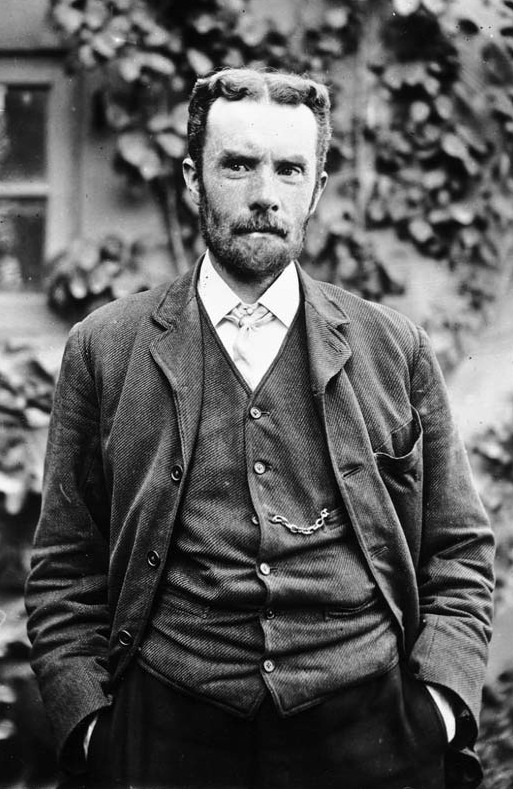
\includegraphics[height=7cm]{oheaviside}
        \caption*{Photograph of Oliver Heaviside, circa 1900.}
        \caption*{Credit Smithsonian Libraries, public domain.}
    \end{subfigure}
    \hfill%
    \begin{subfigure}[t]{.47\textwidth}
        \centering
        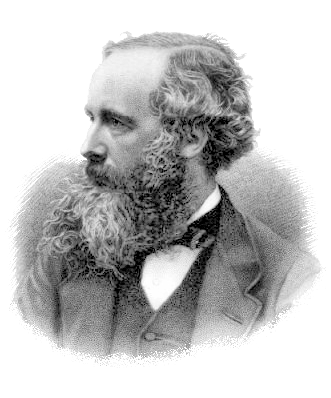
\includegraphics[height=7cm]{jamesclerkmaxwell}
        \caption*{Engraving of James Clerk Maxwell by G. J. Stodart from a photograph by Fergus of Greenock.}
        \caption*{G. J. Stodart - Frontpiece in James Maxwell, The Scientific Papers of James Clerk Maxwell. Ed: W. D. Niven. New York: Dover, 1890.  Public domain.}
    \end{subfigure}%
\end{figure}
